% ---------------------------------------------------------------------------
%  From the Policy Gradient to Self-Play
%  A tutorial monograph on the mathematics of AlphaZero-style reinforcement
%  learning and its implementation in Rust and Burn.
%
%  Build:  pdflatex main && bibtex main && pdflatex main && pdflatex main
%  Engine: pdfLaTeX. Do not use biblatex (biber is not installed).
% ---------------------------------------------------------------------------
\documentclass[11pt,a4paper]{article}

\usepackage[T1]{fontenc}
\usepackage[utf8]{inputenc}
\usepackage{lmodern}
\usepackage[final]{microtype}
\usepackage[margin=2.3cm]{geometry}
\usepackage{amsmath,amssymb,amsthm,mathtools}
\usepackage{booktabs}
\usepackage{array}
\usepackage{tabularx}
\usepackage{listings}
\usepackage{xcolor}
\usepackage{fancyhdr}
\usepackage[hidelinks]{hyperref}
\usepackage[numbers,sort&compress]{natbib}
\usepackage{tikz}
\usetikzlibrary{arrows.meta,positioning,fit,backgrounds,calc}

% --- page style ------------------------------------------------------------
\pagestyle{fancy}
\fancyhf{}
\fancyhead[L]{\small\nouppercase{\leftmark}}
\fancyhead[R]{\small\thepage}
\renewcommand{\headrulewidth}{0.4pt}
\setlength{\parskip}{0.35em}

% --- theorem-like environments --------------------------------------------
\theoremstyle{definition}
\newtheorem{definition}{Definition}[section]
\newtheorem{remark}[definition]{Remark}
\theoremstyle{plain}
\newtheorem{proposition}[definition]{Proposition}
\newtheorem{theorem}[definition]{Theorem}

% --- macros ----------------------------------------------------------------
\newcommand{\E}{\mathbb{E}}
\newcommand{\R}{\mathbb{R}}
\newcommand{\Prob}{\mathbb{P}}
\DeclareMathOperator*{\argmax}{arg\,max}
\DeclareMathOperator*{\argmin}{arg\,min}
\newcommand{\bs}[1]{\boldsymbol{#1}}
\newcommand{\dd}{\mathrm{d}}
\newcommand{\code}[1]{\texttt{#1}}
\newcommand{\tensor}[1]{\mathsf{#1}}

% --- code listings ---------------------------------------------------------
\definecolor{codekw}{RGB}{0,90,160}
\definecolor{codety}{RGB}{120,60,140}
\definecolor{codestr}{RGB}{0,120,80}
\definecolor{codecmt}{RGB}{110,110,110}
\definecolor{codebg}{RGB}{250,250,250}
\definecolor{coderule}{RGB}{210,210,210}

% Listings in TeX Live 2022 (basic scheme) has no Rust language, so it is
% defined here. Keep the keyword list short and stable.
\lstdefinelanguage{RustX}{
  keywords={as,break,const,continue,crate,else,enum,extern,false,fn,for,if,impl,
            in,let,loop,match,mod,move,mut,pub,ref,return,self,Self,static,struct,
            super,trait,true,type,unsafe,use,where,while,async,await,dyn},
  ndkeywords={u8,u16,u32,u64,i8,i16,i32,i64,f32,f64,usize,isize,bool,
              Vec,Option,Result,Some,None,Ok,Err,Box,Rc,RefCell,Arc,Mutex,
              String,Send,Sync,Tensor,Module,Autodiff,Backend},
  sensitive=true,
  comment=[l]{//},
  morecomment=[s]{/*}{*/},
  string=[b]",
  morestring=[b]',
}

\lstdefinestyle{rust}{
  language=RustX,
  basicstyle=\ttfamily\footnotesize,
  keywordstyle=\color{codekw}\bfseries,
  commentstyle=\color{codecmt}\itshape,
  stringstyle=\color{codestr},
  emphstyle=\color{codety},
  numbers=none,
  showstringspaces=false,
  breaklines=true,
  columns=fullflexible,
  keepspaces=true,
  frame=single,
  rulecolor=\color{coderule},
  backgroundcolor=\color{codebg},
  framesep=4pt,
  xleftmargin=3pt,
  aboveskip=0.7em,
  belowskip=0.7em,
}

\lstdefinestyle{plaintext}{
  basicstyle=\ttfamily\footnotesize,
  numbers=none,
  showstringspaces=false,
  breaklines=true,
  columns=fullflexible,
  keepspaces=true,
  frame=single,
  rulecolor=\color{coderule},
  backgroundcolor=\color{codebg},
  framesep=4pt,
  aboveskip=0.7em,
  belowskip=0.7em,
}

\lstdefinestyle{algo}{
  basicstyle=\ttfamily\footnotesize,
  numbers=left,
  numberstyle=\tiny\color{codecmt},
  numbersep=8pt,
  showstringspaces=false,
  breaklines=true,
  columns=fullflexible,
  keepspaces=true,
  frame=single,
  rulecolor=\color{coderule},
  backgroundcolor=\color{codebg},
  framesep=4pt,
  aboveskip=0.8em,
  belowskip=0.8em,
}

% ---------------------------------------------------------------------------
\title{\bfseries From the Policy Gradient to Self-Play\\[0.4em]
\large The mathematics of AlphaZero-style reinforcement learning,\\
\large and the shape it takes in Rust and Burn}
\author{}
\date{\today}

\begin{document}

\maketitle

\begin{abstract}
\noindent
This monograph follows one continuous line of mathematics from its classical
beginnings to a working self-play agent, and then follows the same line into
code. The mathematical part starts with the Markov decision process, the
policy gradient theorem, and the deterministic policy gradient; it continues
through approximate policy iteration and Expert Iteration to the bandit
results that justify tree search. The algorithmic part states the AlphaZero
procedure exactly, gives the reason each component exists, and records which
of its parts have a proof and which rest on experiment. The engineering part
treats two problems that dominate an implementation: the representation of a
search tree in a language without a garbage collector, and the parallel
organisation of self-play against a single shared accelerator. The target
application is freestyle Gomoku under the Swap2 opening rule, in Rust with
the Burn framework; the same shapes apply to any two-player,
perfect-information board game after a change of rules engine.

The monograph is written for readers who know Rust at an intermediate level
and machine learning at a graduate level. It gives derivations rather than
citations alone, and it gives the reasoning behind implementation choices
rather than complete programs. Code fragments are illustrative and
deliberately short.
\end{abstract}

\tableofcontents

\section{Introduction}
\label{sec:intro}

\subsection{What this monograph follows}

There is a single line of mathematics that runs from the definition of a
Markov decision process to a program that teaches itself to play a board game.
This monograph follows that line in one direction, and then follows the same
line into code.

The mathematical path has six steps:

\begin{enumerate}
  \item the \emph{objective} of a parameterized policy, and the likelihood-ratio
        identity that makes its gradient estimable from samples alone
        (Section~\ref{sec:reinforce});
  \item the \emph{policy gradient theorem}, which removes the derivative of the
        state distribution from the gradient (Section~\ref{sec:pgt});
  \item the \emph{actor--critic} decomposition, and the instability that
        bootstrapping introduces (Section~\ref{sec:actorcritic});
  \item the \emph{deterministic policy gradient}, the sibling branch of the same
        idea, and a clarification of its place in the lineage
        (Section~\ref{sec:dpg});
  \item \emph{approximate policy iteration} and its reformulation as Expert
        Iteration, which is the exact frame around the AlphaZero loop
        (Sections~\ref{sec:apxpi} and~\ref{sec:exit});
  \item the \emph{bandit} results that give tree search its exploration rule and
        its only real guarantees (Section~\ref{sec:bandits}).
\end{enumerate}

The algorithmic path has three steps: the sequence of three DeepMind papers that
deleted one crutch at a time (Section~\ref{sec:three-papers}), the algorithm as a
whole including its search and its loss
(Sections~\ref{sec:algorithm}--\ref{sec:loss}), and the honest inventory of which
parts are proven and which are not (Section~\ref{sec:proven}).

The engineering path has two dominant problems, and this is where most of the
implementation effort actually goes:

\begin{itemize}
  \item \textbf{The shape of the search tree in Rust.} A game tree is a
        recursively owned structure, which is the structure the Rust ownership
        model is least willing to express directly. Section~\ref{sec:tree}
        develops the flat-arena representation, states its invariants, and shows
        the traversal pattern that keeps the borrow checker satisfied without
        runtime checks.
  \item \textbf{The parallel organisation of self-play.} Self-play needs
        thousands of position evaluations per second from one accelerator, while
        the tree search that produces them is irregular, branchy, and cheap. The
        answer is to build many independent trees rather than one shared tree, and
        to make the accelerator a batching service at the single point of
        synchronization. Section~\ref{sec:parallel} develops this.
\end{itemize}

\subsection{The target application}

Every concrete example in this monograph uses freestyle Gomoku on a
$15\times15$ board, with the Swap2 opening protocol. Gomoku is a useful target
for three reasons.

First, it is tactically sharp and short. A game lasts roughly 30 to 70 moves,
and single moves decide games. This is the opposite regime from Go, where
influence accumulates slowly over hundreds of moves. The consequence for the
capital---compute, network size, number of self-play games---is large and
favourable: published AlphaZero-style Gomoku agents reached human playing
strength with networks two orders of magnitude smaller than the Go networks
\citep{xie2018alphagomoku}.

Second, the mechanics are simple enough to be fully specified in a page, which
keeps the rules engine small and keeps this monograph's examples short.

Third, and least obviously, Gomoku has a solved core: Allis and colleagues
proved in 1993 and 1994 that freestyle Gomoku on $15\times15$ is a forced win for
the first player \citep{allis1996gomoku,allis1994thesis}. This is a gift rather
than a problem. Board positions of which the exact value is known, and forced
win sequences that can be verified mechanically, are perfect test data for a
search implementation, and they are available before any learning happens. The
competitive variant, which the Swap2 opening rule produces, is not solved
(Section~\ref{sec:solved}), so the agent still plays on open ground.

\subsection{The ``alpha-epsilon'' position}

A pure AlphaZero agent knows nothing about the game except its rules. This
monograph describes a small, deliberate departure from that purity: hand-written
tactical detection (a win in one move, a forced block, a double threat) computed
by bit operations, together with a bounded threat-space prover.

The departure matters for three reasons, and only the first is about strength.
Tactical detection gives the learning curve a head start, because a young
network's priors are nearly uniform and a prior that already points at immediate
wins saves thousands of fruitless self-play games. The same detection code
serves as a deterministic stand-in evaluator, which allows the entire search to
be built, tested, and proven correct before a single gradient is computed. And
the bounded prover produces labelled positions, whose labels are exact rules
truths rather than bootstrap estimates, which a small fraction of every training
batch can then use as an anchor.

The word \emph{epsilon} in the label is the honest part: the hand-written
knowledge is a small perturbation to an otherwise learned system, not a
replacement for it. Section~\ref{sec:alphaepsilon} states exactly what the
component may and may not do.

\subsection{Scope}

This monograph gives derivations for the mathematics and reasoning for the
implementation. It does not give complete programs, complete hyperparameter
sweeps, or benchmark results, and it does not describe any particular
repository. Code fragments are illustrative and are kept below roughly fifteen
lines where possible.

Three things are deliberately out of scope. Reinforcement learning from
imperfect information (poker, simultaneous games) is not covered, because nothing
in the AlphaZero line applies to it without a substantial reformulation.
Continuous control is covered only at the point where the deterministic policy
gradient enters the narrative (Section~\ref{sec:dpg}); it is discussed because
it is frequently confused with the AlphaZero line, and the confusion is worth
clearing. Finally, distributed training across several accelerators is not
covered: the parallel design in Section~\ref{sec:parallel} is explicitly the
single-accelerator design, and the reasons for the choice are stated there.

\subsection{How to read this monograph}

Readers who want the algorithm should read Sections~\ref{sec:three-papers}
through~\ref{sec:loss} and can treat the mathematical section as reference
material. Readers who want to build the system should read
Sections~\ref{sec:tree} and~\ref{sec:parallel} first: those two sections contain
the design decisions that are expensive to change later.

Readers who are following the original papers should note one recurring
distinction. The primary sources publish algorithms and architectures in full
detail but are reticent about constants. Where a constant is not published, this
monograph says so at the point of use, and marks the substitute as an
experimental choice. Table~\ref{tab:folklore} collects these cases, and this is
the most practically useful table in the document.

All symbols are collected in Appendix~\ref{app:notation} and are redefined at
first use in the body.

\begin{table}[t]
\centering
\small
\caption{Constants commonly attributed to the primary sources but not published
by them. The ``actual source'' column names where the number really comes from.}
\label{tab:folklore}
\begin{tabularx}{\textwidth}{@{}l l X@{}}
\toprule
Constant & Commonly claimed source & Actual source \\
\midrule
$c_{\mathrm{puct}} = 1.5$ & AlphaGo Zero / AlphaZero & Not published by DeepMind;
first widely used published value is from \citet{tian2019elf} \\
Replay window size & AlphaZero & Not published; the 500{,}000-game window is
AlphaGo Zero's, reported via \citet{tian2019elf} \\
Dirichlet $\alpha$ & AlphaZero & The rule $\alpha \approx 10 / (\text{typical legal moves})$
is published; the specific per-game values follow from it \\
Simulations per move & --- & 1600 (AlphaGo Zero), 800 (AlphaZero). Do not mix
them \\
Gating threshold 55\% over 400 games & AlphaGo Zero & Removed entirely in
AlphaZero \\
\bottomrule
\end{tabularx}
\end{table}

\section{Mathematical foundations}
\label{sec:foundations}

\subsection{Markov decision processes and the objective}
\label{sec:mdp}

\begin{definition}[Markov decision process]
A \emph{Markov decision process} (MDP) is a tuple
$\mathcal{M} = (\mathcal{S}, \mathcal{A}, P, r, \gamma)$: a set of states
$\mathcal{S}$; a set of actions $\mathcal{A}$; a transition kernel
$P(s' \mid s,a)$; a reward function $r : \mathcal{S} \times \mathcal{A} \to \R$;
and a discount factor $\gamma \in [0,1]$.
\end{definition}

A \emph{policy} maps states to distributions over actions. When the policy is
represented by parameters $\theta$, we write $\pi_\theta(a \mid s)$. The value
functions are

\begin{align}
v^{\pi}(s) &= \E_{\pi}\!\left[\textstyle\sum_{t \ge 0} \gamma^t r_t
\;\middle|\; s_0 = s\right], &
Q^{\pi}(s,a) &= \E_{\pi}\!\left[\textstyle\sum_{t \ge 0} \gamma^t r_t
\;\middle|\; s_0 = s, a_0 = a\right],
\end{align}

and they satisfy the Bellman equations
$v^\pi(s) = \sum_a \pi(a\mid s) Q^\pi(s,a)$ and
$Q^\pi(s,a) = r(s,a) + \gamma \sum_{s'} P(s'\mid s,a)\, v^\pi(s')$.

The \emph{objective} is the expected outcome of the initial states under the
policy,
\begin{equation}
J(\theta) \;=\; \E_{s_0 \sim \rho}\!\left[ v^{\pi_\theta}(s_0) \right],
\label{eq:objective}
\end{equation}
where $\rho$ is the distribution over starting states.

Two specializations are worth stating at once, because the rest of this
monograph uses them exclusively.

\begin{remark}[Two-player perfect-information games as MDPs]
For a deterministic, perfect-information, zero-sum game with two players, the
following hold.
\begin{enumerate}
  \item $\mathcal{S}$ is the set of legal board positions, $\mathcal{A}$ the set
        of legal moves at a position, and $P$ is deterministic: a move
        determines the next position.
  \item The reward is zero at every non-terminal step and equals the game
        outcome at a terminal state. With outcomes in $\{-1, 0, +1\}$ and
        $\gamma = 1$, the return from a terminal state is exactly the game
        result, and every value lies in $[-1,1]$.
  \item The two players' value functions are related by $v(s) = -v(s')$ when
        $s'$ is the position seen by the opponent. This \emph{sign alternation}
        is the single most common source of implementation defects
        (Section~\ref{sec:tree}).
\end{enumerate}
\end{remark}

\subsection{The likelihood-ratio identity, and REINFORCE}
\label{sec:reinforce}

The objective \eqref{eq:objective} is an expectation over trajectories, and
the trajectories depend on $\theta$. The first step of the whole subject is to
make that dependence disappear by differentiating a probability instead of a
value.

Let $\tau = (s_0, a_0, s_1, a_1, \dots, s_T)$ be a trajectory. Its probability
under the policy factorizes:

\begin{equation}
p_\theta(\tau) \;=\; \rho(s_0) \prod_{t=0}^{T-1}
\pi_\theta(a_t \mid s_t)\, P(s_{t+1} \mid s_t, a_t).
\label{eq:trajprob}
\end{equation}

\begin{proposition}[Likelihood-ratio identity]
\label{prop:likelihood-ratio}
For any function $f$ of the trajectory,
$\nabla_\theta\, \E_{\tau \sim p_\theta}[f(\tau)] =
\E_{\tau \sim p_\theta}\!\left[ f(\tau)\, \nabla_\theta \log p_\theta(\tau) \right]$.
\end{proposition}

\begin{proof}
$\nabla_\theta \E[f] = \nabla_\theta \int p_\theta(\tau) f(\tau) \dd\tau
= \int f(\tau) \nabla_\theta p_\theta(\tau) \dd\tau$. Since
$\nabla_\theta p_\theta = p_\theta \nabla_\theta \log p_\theta$, the identity
follows, provided the exchange of derivative and integral is justified; this
requires that $\pi_\theta$ be differentiable in $\theta$ and that the standard
dominated-convergence conditions hold.
\end{proof}

Apply Proposition~\ref{prop:likelihood-ratio} with $f(\tau) = R(\tau)$, the
return of the trajectory. Taking logarithms in \eqref{eq:trajprob}, the initial
state distribution and the transition kernel do not depend on $\theta$, so all
that remains is

\begin{equation}
\nabla_\theta \E[R] \;=\;
\E\!\left[ R(\tau) \sum_{t=0}^{T-1} \nabla_\theta \log \pi_\theta(a_t \mid s_t)
\right].
\label{eq:reinforce}
\end{equation}

This is the REINFORCE estimator \citep{williams1992reinforce}. It needs no
model of $P$: samples and a score function suffice. With a
\emph{return-to-go} refinement, $R(\tau)$ is replaced at step $t$ by
$G_t = \sum_{t'\ge t} \gamma^{t'-t} r_{t'}$, because rewards before time $t$
cannot be affected by $a_t$; the estimator is unchanged in expectation and
lower in variance.

For a board game with $\gamma = 1$ and outcome $z \in \{-1,0,+1\}$, the
return-to-go from any non-terminal step is simply $z$. Equation
\eqref{eq:reinforce} becomes

\begin{equation}
\nabla_\theta J(\theta) \;=\;
\E\!\left[ z \sum_{t} \nabla_\theta \log \pi_\theta(a_t \mid s_t) \right],
\label{eq:reinforce-game}
\end{equation}

that is: raise the log-probability of every move played in a won game, and
lower it in a lost game. This is exactly the reinforcement-learning stage of
AlphaGo (2016) \citep{silver2016alphago}. It is worth holding on to for two
paragraphs, because it is the point at which the popular description of
AlphaZero as ``policy gradient plus search'' goes wrong
(Section~\ref{sec:loss}).

A \emph{baseline} $b(s)$, any function of the state that does not depend on the
action, leaves the estimator unbiased:

\begin{equation}
\E\!\left[ (G_t - b(s_t))\, \nabla_\theta \log \pi_\theta(a_t \mid s_t) \right]
= \nabla_\theta J(\theta),
\label{eq:baseline}
\end{equation}

because $\E_{a \sim \pi}[b(s) \nabla \log \pi(a|s)] = b(s) \nabla \sum_a \pi(a|s)
= b(s) \nabla 1 = 0$. Choosing $b(s_t) = v^{\pi}(s_t)$ turns the multiplier into
an advantage estimate and reduces variance by orders of magnitude in practice;
choosing $b$ as a bootstrapped estimate is the actor--critic idea
(Section~\ref{sec:actorcritic}).

\subsection{The policy gradient theorem}
\label{sec:pgt}

Equation \eqref{eq:reinforce} has a weakness that is not visible in the board-game
setting but is fatal elsewhere: the multiplier $G_t$ is the return of a whole
sampled trajectory, so its variance grows with the horizon. It would be far
better to weight the score function by a local quantity, $Q^\pi(s_t,a_t)$. The
policy gradient theorem says that this is allowed, and that the price is a
change of state distribution.

\begin{theorem}[Policy gradient theorem, \citeauthor{sutton2000policygradient}]
\label{thm:pgt}
For a differentiable policy $\pi_\theta$ and any start-state distribution,
\begin{equation}
\nabla_\theta J(\theta) \;=\;
\sum_{s} d^{\pi}(s) \sum_{a} Q^{\pi}(s,a)\, \nabla_\theta \pi_\theta(a \mid s),
\label{eq:pgt}
\end{equation}
where $d^{\pi}(s) = \sum_{t\ge 0} \gamma^t \Prob(s_t = s)$ is the
discounted state-visitation distribution under $\pi$.
Equivalently,
$\nabla_\theta J(\theta) = \E_{s \sim d^\pi}
\!\left[\sum_a Q^\pi(s,a) \nabla_\theta \pi_\theta(a|s)\right]$.
\end{theorem}

\begin{proof}[Proof sketch]
Write $J(\theta) = \sum_s d_0(s) v^{\pi_\theta}(s)$ and differentiate
$v^{\pi_\theta}$ by unrolling one Bellman step:
\[
\nabla v^{\pi}(s)
= \sum_a \Big[ \nabla \pi(a|s)\, Q^{\pi}(s,a)
  + \pi(a|s) \sum_{s'} P(s'|s,a)\, \gamma\, \nabla v^{\pi}(s') \Big].
\]
Note which terms are missing: $Q^\pi$ is not differentiated. Substitute this
expression into itself repeatedly. Every unrolling multiplies the state
distribution by $\gamma \sum_a \pi(a|s) P(s'|s,a)$, so after infinitely many
unrollings the outer distribution becomes exactly $d^\pi$, and the term
$\nabla \pi$ is collected once at each level. Summing the resulting geometric
series gives \eqref{eq:pgt}.
\end{proof}

The content of the theorem is what the proof sketch reveals: \emph{the
derivative of the state distribution is never needed}. The distribution
$d^\pi$ appears as a weight, not as a function to be differentiated. This is
what makes sample-based estimation possible at all, and it is why
\eqref{eq:reinforce} and \eqref{eq:pgt} agree in expectation: the sample return
$G_t$ is an unbiased estimate of $Q^\pi(s_t,a_t)$ under the same distribution.

Combining \eqref{eq:pgt} with the log-derivative trick gives the practical form

\begin{equation}
\nabla_\theta J(\theta) \;=\;
\E_{s \sim d^\pi,\, a \sim \pi}\!\left[ Q^{\pi}(s,a)\, \nabla_\theta
\log \pi_\theta(a \mid s) \right],
\label{eq:pgt-score}
\end{equation}

which is the same as \eqref{eq:reinforce} except that the multiplier is now a
\emph{state--action value}, not a trajectory return. Any unbiased estimate of
$Q^\pi$ may be substituted; the choice of estimator is the actor--critic design
space.

\subsection{Actor--critic, bootstrapping, and the deadly triad}
\label{sec:actorcritic}

Substituting a learned approximation $Q_w(s,a) \approx Q^\pi(s,a)$ into
\eqref{eq:pgt-score} gives the actor--critic architecture: an \emph{actor}
$\pi_\theta$ that is improved by the gradient, and a \emph{critic} $Q_w$ that
supplies the multiplier. There are two ways to train the critic, and they
differ in a way that decides the whole stability picture.

\paragraph{Monte Carlo.} Use the observed return $G_t$ as the target for
$Q_w(s_t,a_t)$. The target is an unbiased sample of the true value under the
current policy. The variance is high, because a single game outcome is a noisy
estimate of one position's worth; the bias is zero.

\paragraph{Temporal difference.} Use a one-step bootstrap
$\hat{y}_t = r_t + \gamma\, Q_w(s_{t+1}, a_{t+1})$ as the target, and descend on
the squared temporal-difference (TD) error
\begin{equation}
\delta_t \;=\; r_t + \gamma\, Q_w(s_{t+1},a_{t+1}) - Q_w(s_t,a_t).
\label{eq:td}
\end{equation}
The target is biased, because it depends on the same estimate being trained.
The variance is much lower, because it involves one transition rather than a
whole episode. TD learning propagates information backwards through the state
space, which is why it is sample-efficient; but the bias is real, and it becomes
harmful in combination with the next two ingredients.

\begin{remark}[The deadly triad]
Divergence of value estimation is possible when three conditions hold
simultaneously: \emph{function approximation}, \emph{bootstrapping}, and
\emph{off-policy} learning \citep{suttonbarto2018}. Each is individually
manageable. Approximate value functions alone may simply be inaccurate.
Bootstrapping alone is the basis of TD learning. Off-policy learning alone
requires importance weights but is sound. Together they can produce a feedback
loop in which the approximation error of the target feeds the update, which
enlarges the error.
\end{remark}

This remark returns in Section~\ref{sec:alphazero-why}, because one of the
cleanest features of the AlphaZero design is that it removes the second
ingredient completely: the value target is the raw game outcome, so the loop
never bootstraps.

\subsection{The deterministic policy gradient, and the DDPG branch}
\label{sec:dpg}

The policy gradient of Section~\ref{sec:pgt} integrates over actions. For a
discrete game that integration is cheap: the number of legal moves is at most a
few hundred. For a continuous action space it is the dominant cost, and the
usual resolution is to make the policy deterministic.

\begin{definition}[Deterministic policy]
A deterministic policy is a differentiable map
$\mu_\theta : \mathcal{S} \to \mathcal{A}$. Its objective is
\begin{equation}
J(\theta) \;=\; \E_{s \sim \rho^{\mu}}\!\left[ Q^{\mu}\!\left(s, \mu_\theta(s)\right)\right],
\label{eq:dpg-objective}
\end{equation}
where $\rho^\mu$ is the discounted state distribution induced by $\mu_\theta$.
\end{definition}

Because the action is now a deterministic function of the state, the gradient
of the objective with respect to $\theta$ can be taken by the chain rule -- the
action distribution no longer depends on $\theta$ in a way that must be
integrated out.

\begin{proposition}[Deterministic policy gradient, \citeauthor{silver2014dpg}]
\label{prop:dpg}
Under the usual conditions on differentiability and on the existence of
$\rho^\mu$,
\begin{equation}
\nabla_\theta J(\theta) \;=\;
\E_{s \sim \rho^{\mu}}\!\left[
\underbrace{\nabla_\theta \mu_\theta(s)}_{\text{how to move}}
\cdot
\underbrace{\nabla_a Q^{\mu}(s,a)\big|_{a = \mu_\theta(s)}}_{\text{which way is better}}
\right].
\label{eq:dpg}
\end{equation}
\end{proposition}

\begin{proof}[Proof sketch]
Differentiate \eqref{eq:dpg-objective}. Two kinds of term appear: those in which
$\theta$ enters through $\mu_\theta$ inside $Q^\mu$, and those in which $\theta$
enters through the state distribution $\rho^\mu$. The second kind is
$\sum_s \nabla_\theta \rho^\mu(s)\, Q^\mu(s,\mu_\theta(s))$. Using the
consistency identity of the deterministic policy,
$\nabla_\theta \rho^\mu(s) = \rho(s_0)\sum_t \gamma^t \nabla_\theta P(s_t = s)$,
the state-distribution term can be rewritten as
$\sum_t \gamma^t \sum_s \rho(s_0) \nabla_\theta P(s_t = s)
\, Q^\mu(s,\mu_\theta(s))$. This expression vanishes because it is the
derivative of $\sum_s P(s_t = s) = 1$ with respect to $\theta$, dotted with the
constant factor $Q^\mu(s,\mu_\theta(s))$ evaluated at the same $s$; formally,
it is an expectation of a total derivative of a probability and cancels by the
same argument that removes the state-distribution derivative in
Theorem~\ref{thm:pgt}. What remains is the two-factor product
\eqref{eq:dpg}. The full argument, including the conditions, is
\citet{silver2014dpg}.
\end{proof}

The two factors of \eqref{eq:dpg} have a direct reading that is worth keeping:
$\nabla_\theta \mu_\theta(s)$ says how the chosen action changes when the
parameters change, and $\nabla_a Q^\mu$ says which direction in action space
improves the value. Their product is an ascent direction for the value, obtained
without integrating over actions at all.

The theorem also explains the relationship between the two branches. If the
stochastic policy is a fixed-variance Gaussian,
$\pi_\theta(a|s) = \mathcal{N}\!\left(\mu_\theta(s), \sigma^2 I\right)$, then the
stochastic policy gradient of Theorem~\ref{thm:pgt} converges, as
$\sigma \to 0$, to the deterministic gradient \eqref{eq:dpg} plus a term of order
$\sigma^2$ involving the second derivative of $Q$ at the mean. In the limit, only
the deterministic formula survives. That limit is the content of the connection,
and it is the reason a deterministic actor can be trained at all: the gradient
of the value with respect to the action is a usable teaching signal.

\begin{remark}[Attribution, and a correction worth making once]
The deterministic policy gradient is \citet{silver2014dpg}. The deep version of
it -- an off-policy actor--critic with a replay buffer, target networks, and
action-noise exploration, which is the algorithm usually called \emph{deep
deterministic policy gradient} or DDPG -- is \citet{lillicrap2015ddpg}, whose
author list begins with Lillicrap and Hunt and ends with Silver and Wierstra.
Silver is a co-author of DDPG, not its author, and DDPG is not the parent of
AlphaGo: it is a parallel branch. The two branches share the actor--critic
frame, the chain rule through the action, and nothing else that matters. DDPG
exists because continuous actions make a stochastic policy expensive to
integrate over; AlphaZero exists because discrete games make a lookahead search
cheap to run. DDPG learns a bootstrapped critic $Q_w$ and must inject
exploration noise into a deterministic actor. AlphaZero learns no critic at all:
the search supplies local action values, the value head supplies $v$, and the
target is never bootstrapped. Section~\ref{sec:three-papers} resumes the
AlphaZero branch and does not use DDPG again.
\end{remark}

\subsection{Approximate policy iteration}
\label{sec:apxpi}

Classical policy iteration alternates two steps in an exact MDP:

\begin{enumerate}
  \item \textbf{Policy evaluation}: compute $v^{\pi}$ for the current policy.
  \item \textbf{Policy improvement}: set $\pi'(s) = \argmax_a Q^{\pi}(s,a)$.
\end{enumerate}

The guarantee for the second step is the improvement theorem: acting greedily
with respect to the value of a policy produces a policy that is at least as
good everywhere, and strictly better wherever the greedy action improves on the
policy's own action \citep{suttonbarto2018}. Because the number of deterministic
policies in a finite MDP is finite and the sequence is monotonically improving,
policy iteration converges to an optimal policy in finitely many iterations.

Both steps become approximations as soon as the state space is large. The
improvement step still requires a maximization over actions -- cheap in a
discrete game, impossible in a continuous one -- and the evaluation step
requires a function approximator. The resulting scheme, \emph{approximate policy
iteration}, has no general convergence guarantee, and there are classical
counterexamples.

The AlphaZero loop is an approximate policy iteration, and the AlphaGo Zero
paper states exactly this:

\begin{quote}
``The AlphaGo Zero self-play algorithm can be understood as an approximate
policy iteration scheme in which MCTS is used for both policy improvement and
policy evaluation'' \citep{silver2017alphagozero}.
\end{quote}

The mapping onto the two steps is as follows.

\emph{Improvement} is the tree search. Given the network's policy $p$ and value
$v$, the search returns a distribution $\pi$ over the root's moves. That
distribution is what the network's policy would become if it could look ahead:
it is a better policy than $p$, for the same reasons a greedy step on an
accurate $Q$ is better than the policy that generated the $Q$.

\emph{Evaluation} is the value head trained on $z$, the outcome of games played
with the improved policy. There is no separate critic; the value network is
retrained on outcomes generated by the improved policy, which is precisely the
policy-evaluation step of the loop.

The loop is then: improve with search, evaluate by training on outcomes of the
improved policy, re-derive the policy from the improved network, repeat. The
structural reason it does not stall at the network's own level is the asymmetry
between the two actors: the teacher (the search, which uses the network as a
prior and as a leaf evaluator) is stronger than the student (the network alone),
because the search corrects the network's errors by lookahead and by comparing
alternatives. Every iteration distils that correction back into the weights,
which raises the level at which the next search operates.

\subsection{Expert Iteration}
\label{sec:exit}

The cleanest theoretical frame for the loop is \emph{Expert Iteration} (ExIt),
introduced by \citet{anthony2017exit}. It separates the two roles explicitly.

A \emph{apprentice} is a function approximator $\pi_\theta$ that imitates
decisions. An \emph{expert} is a planner that improves upon the apprentice by
lookahead and returns a better decision distribution. Expert Iteration repeats
one step: plan with the expert on states, then refit the apprentice to the
expert's improved decisions. Formally, with an expert operator
$E(\pi_\theta)$ that maps a policy to a better one,

\begin{equation}
\pi_{\theta} \;\longmapsto\; E(\pi_\theta) \;\longmapsto\;
\argmin_{\theta'} D\!\left(E(\pi_\theta) \, \|\, \pi_{\theta'}\right)
\;\longmapsto\; \pi_{\theta'}, \qquad \text{repeat.}
\label{eq:exit}
\end{equation}

\citet{anthony2017exit} prove that in the exact, tabular case -- an exact expert
and an unrestricted apprentice -- this iteration converges to the optimal policy.
The proof is a polytope argument: the expert's improvement step is a contraction
in a suitable norm, and the imitation step is exact in the tabular case, so the
sequence of policies is monotone.

AlphaGo Zero is Expert Iteration with MCTS as the expert and a residual
convolutional network as the apprentice. Everything the proof needs is lost in
that instantiation: the expert is an approximation (a finite number of
simulations), the apprentice is a deep network with a fixed architecture, the
data distribution moves with the weights, and the imitation target is stochastic.
The value network has no counterpart in ExIt at all; it is an addition that
supplies the expert with a leaf evaluation. The frame is nevertheless the right
one, because it names the two moving parts, and because it identifies exactly
which assumption each practical departure violates. Section~\ref{sec:proven}
returns to this inventory.

\subsection{Bandits, UCT, and PUCT}
\label{sec:bandits}

Tree search in the AlphaZero line is a sequence of bandit problems, one per
node. This is the mathematical content behind the selection rule; the rest of
the search is bookkeeping.

\paragraph{The bandit problem.} In a $K$-armed bandit, a player chooses one of
$K$ options at each of $n$ rounds and observes a bounded reward from the chosen
option. The quality of a strategy is its \emph{regret}: the expected difference
between the reward of always playing the best arm and the reward actually
collected. The problem is the canonical formalization of the
exploration--exploitation trade-off.

\paragraph{UCB1.} \citet{auer2002ucb1} give the rule
\begin{equation}
a_n \;=\; \argmax_{a}\,\left[\, \bar{Q}_a \;+\;
\sqrt{\frac{2 \ln n}{n_a}} \,\right],
\label{eq:ucb1}
\end{equation}
where $\bar{Q}_a$ is the sample mean reward of arm $a$ and $n_a$ its number of
plays. The first term exploits; the second explores, shrinking as $n_a$ grows and
growing as the total number of plays $n$ grows. UCB1 has logarithmic regret per
arm, and the proof is a concentration argument: the exploration bonus is the
width of a confidence interval for $\bar{Q}_a$ at the required confidence level,
and an arm that could still be optimal is never ruled out permanently.

\paragraph{UCT.} \citet{kocsis2006uct} apply the UCB1 rule at every node of a
search tree instead of at a single bandit. A node's "arms" are its actions, the
"reward" of an arm is the value of the state reached by it, and the values are
backed up along the path to the root. The resulting algorithm is Upper Confidence
bounds applied to Trees (UCT). Its theoretical attraction is a consistency
result: as the number of simulations grows without bound, UCT's root decision
converges to the minimax value, with finite-sample error bounds. UCT is the
algorithm that made Monte Carlo Tree Search (MCTS) work in Go, a domain in which
alpha--beta search had failed for decades \citep{coulom2006mcts, browne2012survey}.

\paragraph{PUCT.} The published AlphaGo Zero selection rule adds a learned prior
to the exploration bonus \citep{rosin2011puct}:

\begin{equation}
a^{*} \;=\; \argmax_a \left[\, Q(s,a) \;+\; c_{\mathrm{puct}}\,
P(s,a)\, \frac{\sqrt{\sum_b N(s,b)}}{1 + N(s,a)} \,\right].
\label{eq:puct}
\end{equation}

The three factors of the exploration bonus each do a job. $P(s,a)$ is the prior
supplied by the network's policy head: it concentrates the search where the
network believes the good moves are. $\sqrt{\sum_b N(s,b)}$ makes the bonus grow
as the node is visited more often, so that a node is never abandoned. The
denominator $1 + N(s,a)$ makes the bonus shrink for the specific arm that has
been tried. The sum form of the growth term is the substantive difference from
UCB1: \emph{any} sibling's visit raises the bonus for \emph{this} arm, so
unexplored arms of a heavily visited node keep attracting attention, and the
sequence of unvisited arms is enumerated rather than sampled at random.

The practical difference between UCT and PUCT is the cost of finding out which
arms are good. The classical UCB1 bonus has to spend visits to estimate every
arm's mean, because it starts from total ignorance. In a game with 150 legal
moves, most of which lose immediately or do nothing, that is most of the budget
spent on distinguishing near-equal bad arms. A prior that is even roughly right
focuses the budget on the few moves that matter, and the whole search becomes
deeper instead of wider.

\begin{remark}[What the prior costs, theoretically]
The guarantee does not survive the prior. UCT's consistency proof needs the
exploration term to be a genuine confidence sequence for an agnostic estimator.
Once $P(s,a)$ comes from a learned function of the position, the bonus is no
longer calibrated to any confidence level, and it can be systematically wrong.
There is no published regret bound or consistency proof for PUCT with learned
priors. This is not a defect of the implementation; it is the state of the
theory, and Section~\ref{sec:proven} states it plainly.
\end{remark}

\paragraph{Proven values.} One classical refinement does carry over intact and is
used directly in this monograph. \citet{winands2008solver} observe that some
nodes have values that are \emph{exact}: a node whose game is over, or a node
whose value has been proven by a sound argument, does not need estimation. Their
MCTS-Solver propagates such values explicitly and stops sampling them. This is
the mechanism that lets a search recognise a forced win, and it is the same
mechanism that lets hand-written tactical detection feed exact labels into
training (Section~\ref{sec:alphaepsilon}).

\subsection{What is proven, and what is not}
\label{sec:proven}

The results collected in this section have very different status, and mixing them
is the most common way to overstate the strength of an AlphaZero-style system.
Table~\ref{tab:proven} separates them.

\begin{table}[t]
\centering
\small
\caption{Status of the results used by an AlphaZero-style agent. The last three
entries are the reason the systems work in practice; they are not theorems.}
\label{tab:proven}
\begin{tabularx}{\textwidth}{@{}X l@{}}
\toprule
Claim & Status \\
\midrule
UCB1 achieves logarithmic regret \citep{auer2002ucb1} & proven \\
UCT converges to the minimax value \citep{kocsis2006uct} & proven \\
Policy gradient with function approximation converges to a local
optimum \citep{sutton2000policygradient} & proven \\
The policy improvement theorem (greedy step does not harm the policy)
\citep{suttonbarto2018} & proven \\
Deterministic policy gradient formula \citep{silver2014dpg} & proven \\
Expert Iteration converges to the optimum \citep{anthony2017exit} & proven,
exact tabular case only \\
PUCT with learned priors converges & \textbf{not proven} \\
Approximate policy iteration with deep function approximation converges
& \textbf{not proven} \\
The AlphaZero loop (deep network $+$ MCTS $+$ self-play) converges
& \textbf{not proven} \\
\bottomrule
\end{tabularx}
\end{table}

Two consequences follow, and they shape the engineering in the rest of this
monograph. First, the guarantees that do exist are guarantees about the
\emph{skeleton} -- a bandit rule, an exact policy iteration, an exact expert.
Every component that makes the system practical breaks an assumption of those
proofs. Second, and consequently, correctness in an implementation must be
established by testing against known facts rather than by appeal to theory. In
the Gomoku setting, known facts are abundant: positions with exact values, and
forced-win sequences that can be verified mechanically. Section~\ref{sec:tree}
uses both.

\section{The AlphaZero algorithm}
\label{sec:alphazero}

\subsection{Three papers, and what each one removed}
\label{sec:three-papers}

The AlphaZero design did not appear at once. It is the residue of three papers,
each of which deleted components that the field believed were necessary, and each
deletion made the system both simpler and stronger. Table~\ref{tab:removals}
records the sequence; the direction of travel is the message.

\begin{table}[t]
\centering
\small
\caption{What each paper removed. Every entry in the first column is a component
that a specialist would have defended before the following paper appeared.}
\label{tab:removals}
\begin{tabularx}{\textwidth}{@{}l l l l@{}}
\toprule
& AlphaGo (2016) & AlphaGo Zero (2017) & AlphaZero (2018) \\
\midrule
Human game data      & yes (supervised policy) & removed & not used \\
Networks             & 3 learned $+$ SL policy  & 1 with two heads & 1 with two heads \\
Handcrafted features & some & removed & removed \\
Random rollouts      & yes (fast policy) & removed & removed \\
Symmetry exploitation & --- & augmentation, averaging & removed \\
Best-network gating  & --- & 55\% gate & removed \\
Games supported      & Go & Go & chess, shogi, Go \\
\bottomrule
\end{tabularx}
\end{table}

\paragraph{AlphaGo (2016).} The system was a pipeline: a supervised policy
network trained on human games, refined by policy-gradient self-play
\eqref{eq:reinforce-game}; a separate value network; a fast rollout policy of
hand-crafted features; and MCTS that combined all four
\citep{silver2016alphago}. It beat Fan Hui 5--0 and Lee Sedol 4--1.

\paragraph{AlphaGo Zero (2017).} Human data, rollouts, hand-crafted features, and
the separate networks were all deleted. One network with two heads, one search,
and a self-play loop remained. After three days of training it beat the
Lee-beating version 100 games to 0; after 40 days it reached an Elo of 5{,}185,
against 4{,}858 for the strongest previous version and 3{,}739 for AlphaGo Lee.
The raw network, with no search at all, measured 3{,}055 \citep{silver2017alphagozero}.
That last number is worth pausing on: it means the network alone, playing a move
per forward pass, was already at the level of a distributed system that used 176
GPUs.

\paragraph{AlphaZero (2018).} The gate, the symmetry exploitation, and the
assumption of binary outcomes were removed, giving one algorithm, one
architecture, and one set of hyperparameters for three games
\citep{silver2018alphazero}. It beat Stockfish after 4 hours, Elmo after 2 hours,
and AlphaGo Lee after 8 hours of training.

\subsection{The algorithm}
\label{sec:algorithm}

\subsubsection{The network}

One network computes both outputs:
\begin{equation}
f_\theta(s) \;=\; (p, v), \qquad
p_a \approx \Prob(a \mid s), \qquad v \approx \E[z \mid s],
\end{equation}
where $s$ is the position, $p$ is a distribution over moves, $v \in [-1,1]$ is
the expected outcome from the side to move, and $z$ is the final outcome of the
game. A single forward pass therefore supplies everything the search needs: a
prior over moves and an evaluation of the position.

\subsubsection{The search}

Each move is chosen after a fixed budget of simulations (1{,}600 in AlphaGo Zero,
800 in AlphaZero; the numbers must not be mixed). One simulation has three
phases, and the difference from classical MCTS is in the second.

\begin{description}
  \item[Select.] Descend from the root, at each node choosing the action of
        \eqref{eq:puct}, until reaching a leaf. A leaf is either terminal or
        never-expanded.
  \item[Expand and evaluate.] If the leaf is terminal, its value is the true game
        outcome, and the network is not called. Otherwise, evaluate it once:
        $(p,v) = f_\theta(s_L)$, store $p$ as the priors of the leaf's outgoing
        edges, and use $v$ as the leaf's value. \emph{There are no rollouts.}
        This is the whole of the replacement of AlphaGo's rollout policy: one
        trained evaluation instead of several hundred random moves.
  \item[Back up.] Propagate $v$ to the root, incrementing visit counts and
        accumulating values along the way. The sign alternates at each ply,
        because the game is zero-sum and the players alternate
        (Section~\ref{sec:tree} takes this up as an implementation matter).
\end{description}

After a move is played, the subtree under the played edge becomes the new root;
the accumulated statistics survive, which is free depth at the next decision.

\subsubsection{Self-play data generation}

Self-play games are generated with the current network guiding the search, with
two exploration mechanisms active at the root.

\emph{Dirichlet noise} perturbs the root priors:
\begin{equation}
P(s_{\mathrm{root}}, a) \;=\; (1-\varepsilon)\, p_a + \varepsilon\, \eta_a,
\qquad \eta \sim \mathrm{Dir}(\alpha), \qquad \varepsilon = 0.25 .
\label{eq:dirichlet}
\end{equation}
AlphaGo Zero used $\alpha = 0.03$ for Go. AlphaZero scaled $\alpha$ in inverse
proportion to the typical number of legal moves: $0.3$ for chess, $0.15$ for
shogi, $0.03$ for Go \citep{silver2018alphazero}. The paper's reason is that the
noise ensures every move may be tried while the search may still overrule bad
moves. A small $\alpha$ produces a spiky noise vector, so a few random moves
receive a large boost per game and different games explore different lines.

\emph{Temperature} controls how the played move is sampled from the visit counts:
\begin{equation}
\pi_a \;\propto\; N(s_{\mathrm{root}}, a)^{1/\tau}.
\label{eq:temperature}
\end{equation}
For the first 30 moves of each AlphaGo Zero game, $\tau = 1$, so play is
proportional to visit counts and openings diversify. Afterwards $\tau \to 0$,
which means playing the most-visited move. The asymmetry is deliberate: early
diversity widens the state distribution that the value head sees, while late
greediness keeps the value target informative, because a game thrown away by
random midgame play teaches the value head very little.

Each position of a finished game is stored as a triple $(s, \pi, z)$, where
$\pi$ is the full visit-count distribution at the root -- not the move that was
played -- and $z$ is the final outcome from the perspective of the player to move
at $s$. AlphaGo Zero additionally applied a random element of the board's
dihedral symmetry group to $s$; AlphaZero removed that step because chess and
shogi have no such symmetry.

AlphaGo Zero also resigned games in which the value estimate stayed below a
threshold, with the false-positive rate held at or below 5\% by forcing 10\% of
games to be played to the end for calibration \citep{silver2017alphagozero}.

\subsubsection{The training step}

Mini-batches are drawn uniformly from a replay window of recent self-play games
(500{,}000 games in AlphaGo Zero; AlphaZero's window size is not published). For
a sample $(s,\pi,z)$ with network output $(p,v)$ the loss is

\begin{equation}
\ell(\theta) \;=\; \underbrace{(z-v)^2\vphantom{\big|}}_{\text{value}}
\;-\; \underbrace{\pi^{\!\top} \log p\vphantom{\big|}}_{\text{policy}}
\;+\; \underbrace{c\,\|\theta\|^2\vphantom{\big|}}_{\text{regularization}},
\qquad c = 10^{-4}.
\label{eq:alphazero-loss}
\end{equation}

The two error terms carry equal weight. AlphaGo Zero justifies this in one
parenthesis: it is reasonable because the rewards are unit-scaled, $r \in
\{-1,+1\}$ \citep{silver2017alphagozero}. Section~\ref{sec:loss} unpacks that
sentence. The optimizer is stochastic gradient descent with momentum $0.9$; the
learning-rate schedules are in Table~\ref{tab:hyper}.

\subsubsection{The outer loop}

AlphaGo Zero ran iterations with a gate: generate games, train a candidate, and
promote the candidate only if it won at least 55\% of 400 evaluation games
against the current best. AlphaZero removed the gate, always training on data
from the latest network. The cost of the gate is compute plus the training steps
spent waiting; the benefit is that a bad network never generates training games.
Removing it was shown to be safe at scale, in part because the replay window
mixes data from many recent checkpoints, so a transient regression dilutes
rather than dominates \citep{tian2019elf,wu2019katago}.

\begin{figure}[t]
\centering
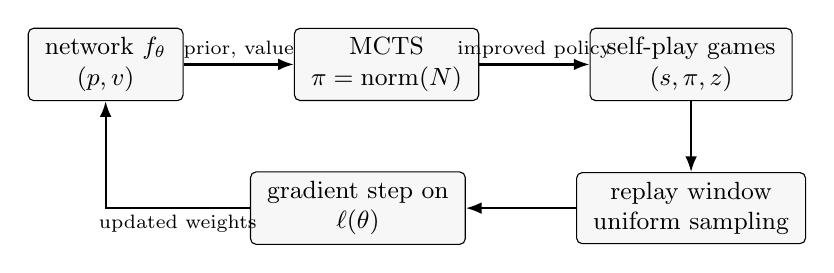
\begin{tikzpicture}[
  node distance=9mm and 14mm,
  box/.style={draw, rounded corners=2pt, align=center, font=\small,
              minimum height=9mm, inner xsep=6pt, fill=black!3},
  arr/.style={-{Latex[length=2mm]}, thick},
  lbl/.style={font=\scriptsize, inner sep=2pt},
]
\node[box] (net) {network $f_\theta$\\$(p,v)$};
\node[box, right=of net] (search) {MCTS\\$\pi = \mathrm{norm}(N)$};
\node[box, right=of search] (games) {self-play games\\$(s,\pi,z)$};
\node[box, below=of games] (buffer) {replay window\\uniform sampling};
\node[box, left=of buffer] (train) {gradient step on\\$\ell(\theta)$};
\draw[arr] (net) -- node[lbl,above]{prior, value} (search);
\draw[arr] (search) -- node[lbl,above]{improved policy} (games);
\draw[arr] (games) -- (buffer);
\draw[arr] (buffer) -- (train);
\draw[arr] (train) -| node[lbl,below,pos=0.25]{updated weights} (net);
\end{tikzpicture}
\caption{The AlphaZero loop. The network is trained to imitate the search; the
improved network then produces a stronger search. Everything else in the system
is engineering around this cycle.}
\label{fig:loop}
\end{figure}

\subsection{Why the loop works}
\label{sec:alphazero-why}

\paragraph{The skeleton is approximate policy iteration.} Section~\ref{sec:apxpi}
already made this identification. The search is the improvement operator, the
value head trained on $z$ is the evaluation operator, and the network is refitted
to both. What makes the loop climb is the asymmetry: the teacher is stronger than
the student, because the teacher is the student plus search.

\paragraph{The value target is the raw game result.} There is no term of the form
$v(s) \leftarrow r + v(s')$. The consequences are worth listing, because they
explain most of the stability of the method.

\emph{Unbiased targets}: $z$ is a sample of the true outcome under the current
improved policy, so it carries no approximation error. \emph{No deadly triad}:
the instability of Section~\ref{sec:actorcritic} requires bootstrapping, and
bootstrapping is absent, so the triad cannot form. \emph{Variance}: a single game
outcome is a noisy estimate of a position's worth; the cure is volume, namely
tens of millions of games and a replay window that averages the noise across each
batch. The team judged unbiased targets worth the variance, in a class of games
where exploration noise must come from the search rather than from dice. KataGo
kept the same choice \citep{wu2019katago}.

\paragraph{The policy target is a distribution.} Training uses $\pi$, the full
visit-count distribution at the root, not the move played. Three arguments
support this. It is an information-dense target: $\pi$ encodes the search's
opinion about every legal move, including how strongly the alternatives were
rejected, while an argmax target keeps one bit of relative preference. This is
the same argument as soft targets in knowledge distillation
\citep{hinton2015distillation}: the relative probabilities of the wrong answers
carry most of the teaching signal. It is a low-variance target, because it
averages hundreds of simulations. And it is by construction the output of the
improvement operator, so imitating it is exactly the imitation step of the
policy-iteration loop.

\paragraph{MCTS averages network errors; minimax amplifies them.} This is the
AlphaZero paper's own argument for why search and deep evaluation fit together,
and it is worth quoting in full:

\begin{quote}
``MCTS averages over these approximation errors, which therefore tend to cancel
out when evaluating a large subtree. In contrast, alpha--beta search computes an
explicit minimax, which propagates the biggest approximation errors to the root
of the subtree'' \citep{silver2018alphazero}.
\end{quote}

A deep network's value errors are confident and hard to predict. Plug such an
evaluator into minimax and the max operator systematically seeks out the largest
errors, because the maximum of a set of noisy estimates is biased upward. MCTS
averages evaluations over many leaf visits, so independent errors partially
cancel. The search is not merely compatible with the network; it is the search
whose error model matches the network's failure mode.

\paragraph{Knowledge replaces computation.} Deleting the rollouts replaced a
cheap, biased, high-variance estimate with one forward pass that returns a
calibrated expectation. The aggregate effect is visible in the search statistics:
in chess AlphaZero searches about 80{,}000 positions per second while Stockfish
searches about 70 million, and in shogi the numbers are 40{,}000 against 35
million \citep{silver2018alphazero}. AlphaZero wins with roughly three orders of
magnitude less search, because each of its evaluations carries learned knowledge
instead of statistics over random play. Breadth is traded for depth of
evaluation, and nothing in the algorithm depends on how fast random rollouts can
be made -- which is also why the algorithm transfers between games.

\paragraph{Self-play is an automatic curriculum.} The opponent is always exactly
as strong as the learner. Early games are between near-random players and are
short and tactically simple; as the network improves, so does the opposition, and
the data always sits at the edge of current ability, which is the regime where
the gradient signal is richest. There is no distribution shift between training
and deployment, because both are self-play. The exploration mechanisms of
Section~\ref{sec:algorithm} exist to prevent the data from collapsing onto a
single deterministic line, which would starve the value head.

\paragraph{Evidence that the loop discovers rather than imitates.} During AlphaGo
Zero training the system rediscovered human joseki, the corner patterns developed
over centuries of play, and then abandoned several of them in favour of variants
it preferred \citep{silver2017alphagozero}. Human knowledge appeared as a
transient phase rather than as a ceiling.

\subsection{Architecture}
\label{sec:architecture}

\paragraph{Input as a stack of planes.} AlphaGo Zero represents a position as a
$19\times19\times17$ image: eight planes for the current player's stones at time
steps $t \dots t-7$, eight for the opponent's, and one constant plane for the
side to move \citep{silver2017alphagozero}. The plane representation is not
incidental. A board is a grid, so the state is an image; the rules are
translation-invariant, which matches weight sharing; they are defined through
adjacencies, which matches local receptive fields; and they are invariant under
rotation and reflection, which matches data augmentation. The paper states this
reasoning explicitly. The history planes supply the temporal context
(repetitions, ko-like situations) that a single snapshot cannot show.

AlphaZero generalized the encoding per game \citep{silver2018alphazero}: keep the
eight-step history, and replace ``stone or no stone'' with one plane per piece
type. Chess needs 6 piece types per side plus 2 repetition planes, times 8
history steps, plus 7 constant planes -- 119 planes per cell. The organizing
principle survived unchanged, and the plans are always oriented to the side to
move, which halves the state space.

\paragraph{Trunk and heads.} The AlphaGo Zero trunk is a convolutional block of
256 filters of size $3\times3$ followed by batch normalization and a rectifier,
then 19 or 39 residual blocks, each of the form
$\mathrm{conv}\,3{\times}3 \to \mathrm{BN} \to \mathrm{ReLU} \to
\mathrm{conv}\,3{\times}3 \to \mathrm{BN} \to (+ \mathrm{skip}) \to \mathrm{ReLU}$

\citep{silver2017alphagozero}. The policy head is a $1\times1$ convolution with
two filters, batch normalization, a rectifier, and a linear layer to one logit
per move; the value head is a $1\times1$ convolution with one filter followed by
linear layers to 256 and then to 1, with a $\tanh$ output.

Two details are load-bearing. The heads are deliberately tiny next to the trunk:
the $1\times1$ convolutions collapse 256 channels to almost nothing before the
expensive linear layers, because the knowledge is expected to live in the shared
body. And the $\tanh$ bounds $v$ to the range of $z$, which keeps the squared
error well scaled and prevents occasional large logits from producing large
gradients.

\paragraph{Why the residual tower, and why one tower for two heads.} The
architecture is the ResNet design \citep{he2016resnet} transplanted from image
classification, and the paper says the hyperparameters were chosen to match the
state of the art in image recognition. Two arguments matter.

Residual connections make very deep networks trainable at all: without them
gradients vanish and training accuracy degrades with depth. And the choice was
measured rather than assumed. AlphaGo Zero trained four architectures on the same
fixed dataset of self-play games \citep{silver2017alphagozero}: one residual
tower with both heads; two residual towers, one per task; one non-residual
convolutional tower with both heads; and two non-residual towers. The first won.
The residual tower accounts for more than 600 Elo, and combining policy and value
into one network accounts for roughly another 600 Elo. The paper reports that
the combination slightly reduced move-prediction accuracy while reducing value
error and raising playing strength, and explains it as regularization to a common
representation that serves multiple use cases.

Two mechanisms produce that effect. Computationally, MCTS needs both outputs at
every leaf, so two separate towers would cost two forward passes per leaf, which
is the dominant cost of self-play. Statistically, the value task forces the trunk
to encode features that predict the outcome while the policy task forces it to
encode features that discriminate good moves from bad; neither task alone needs
the full concept set of the other, but a shared trunk must serve both, so it
learns the union. Each objective trains the other's features. The small drop in
raw move-prediction accuracy is the signature of the trade: a little policy fit
is given up for a lot of position understanding, and playing strength follows
position understanding.

\paragraph{Action encoding.} Go uses a flat distribution over the board plus a
pass move, which does not generalize to games with structured moves. AlphaZero
encodes chess moves as an $8\times8\times73$ stack -- 56 queen-move planes, 8
knight-move planes, 9 underpromotion planes -- giving 4{,}672 moves, and shogi as
$9\times9\times139$ \citep{silver2018alphazero}. Keeping the output spatial, so
that a move means ``from this square, in this direction, by this much'',
preserves the same translation symmetry that helps the input. The price is a
fixed maximal move set, with illegal moves masked and renormalized at search
time. For a game whose moves are simply ``place a stone on an empty cell'' the
flat encoding is already spatial: one output per cell, masked to the legal cells.

\subsection{The loss, term by term -- and why it is not a policy gradient}
\label{sec:loss}

Equation \eqref{eq:alphazero-loss} has three terms with three jobs.

\paragraph{$(z-v)^2$: policy evaluation.} Fit the value head to the true outcome
of games played by the improved policy. The paper treats $v$ as an expectation,
$v \approx \E[z \mid s]$, and mean squared error is the natural fit for an
expectation of a bounded scalar. It preserves the unit-scale argument that
justifies equal weighting, and it accommodates the draw value $0$ without a
reparametrization.

\paragraph{$-\pi^{\!\top}\log p$: policy improvement, written as distillation.}
Cross-entropy between the search distribution and the network policy. Its
minimizer is $p = \pi$: the network is asked to reproduce the search's output for
every move, not only for the move played. This is the term that makes the loop
climb, because $\pi$ is the output of an improvement operator, so fitting $\pi$
pulls the network above its own raw-policy level at every iteration, with
supervision generated on the fly.

\paragraph{$c\|\theta\|^2$: smoothness, with a system-level purpose.} In this
system the regularizer does more than prevent overfitting. MCTS trusts the
network: the prior steers selection and the value steers backup. A network that
overfits the replay window becomes locally erratic -- priors spike on memorized
positions, values swing between neighbouring positions -- and the search built on
top of it degrades, which degrades the next batch of data. Weight decay keeps the
function smooth, which keeps the search meaningful, which keeps the data stream
healthy. The regularizer protects the loop, not only the fit.

\paragraph{What is deliberately absent.} The loss is also defined by what it does
not contain: no bootstrapped term, so targets stay unbiased; no entropy bonus,
because exploration is the search's job
(Section~\ref{sec:alphaepsilon} explains how that separation is kept); no
importance weights, because the replay window is fresh enough for the
policy-iteration framing; and \emph{no policy-gradient term at all}. The
reinforcement-learning signal enters through the data -- the search results --
and not through the gradient estimator.

This last point is the one that is most often misstated. AlphaZero does not
estimate $\nabla_\theta J$ by any method resembling REINFORCE. It runs policy
iteration and supervises the pieces. The policy-gradient layer of
Section~\ref{sec:pgt} is the historical ancestor: it is what trained AlphaGo's
reinforcement-learning policy network in 2016 \eqref{eq:reinforce-game}. By 2017
the explicit gradient step was gone, replaced by distillation from search. The
object being optimized is still the expected outcome of a parameterized policy,
and the convergence intuition still comes from the policy gradient theorem, but
the mechanism is a supervised-fit-to-improved-targets loop. That difference is
why the method trains stably at scales where direct policy-gradient methods are
fragile.

\subsection{Hyperparameters}
\label{sec:hyper}

Table~\ref{tab:hyper} collects the published numbers. It is short on purpose:
the papers specify the algorithm in full and the constants barely at all.

\begin{table}[t]
\centering
\small
\caption{Published training quantities. Where a value is absent, the primary
source does not publish it, and the substitute must be treated as an experiment.
Simulations per move are 1{,}600 in AlphaGo Zero and 800 in AlphaZero; the two
must not be mixed.}
\label{tab:hyper}
\begin{tabularx}{\textwidth}{@{}l X X@{}}
\toprule
Quantity & AlphaGo Zero & AlphaZero \\
\midrule
Residual blocks & 20 (3-day), 40 (40-day) & 19 \\
Channels & 256 & 256 \\
Mini-batch & 2{,}048 & 4{,}096 \\
Training steps & 700k (3-day), 3.1M (40-day) & 700k (mini-batches) \\
Self-play games & approx.\ 4.9M & 44M chess, 24M shogi, 21M Go \\
Learning rate & $10^{-2} \to 10^{-3} \to 10^{-4}$ &
$0.2 \to 0.02 \to 0.002 \to 0.0002$ \\
Optimizer & SGD, momentum 0.9 & SGD, momentum 0.9 \\
Weight decay & $10^{-4}$ (inside the loss) & $10^{-4}$ (inside the loss) \\
Replay window & 500{,}000 games & not published \\
$c_{\mathrm{puct}}$ & not published & not published (1.5 is ELF's value) \\
Dirichlet $\varepsilon$ & 0.25 & 0.25 \\
Dirichlet $\alpha$ & 0.03 (Go) & 0.3 chess, 0.15 shogi, 0.03 Go \\
Temperature & $\tau = 1$ for 30 moves, then $\to 0$ & same form \\
Gating & 55\% over 400 games & removed \\
Hardware & 64 GPU workers $+$ 19 CPU servers & 5{,}000 TPUv1 self-play, 64 TPUv2 train \\
\bottomrule
\end{tabularx}
\end{table}

\subsection{The longer history: a decade of deletions}
\label{sec:history}

The design looks inevitable in hindsight, which it was not. It is the residue of
roughly ten years of removing one crutch at a time \citep{silver2009thesis}.
In 2007, reinforcement learning over hand-crafted local pattern features produced
weak amateur play in Go: local patterns alone do not scale. In 2007--2008,
combining UCT with learned pattern priors produced the first dan-level Go
program, which established that learned knowledge inside tree search multiplies
strength \citep{gelly2007rave}. In 2015, deep Q-networks showed that a single
convolutional network trained from pixels could reach human level on a suite of
Atari games \citep{mnih2015dqn}; the result demonstrated that deep function
approximation is stable enough for reinforcement learning, and it is what made
the following step plausible. It also showed the limits of the value-only
approach: DQN learns a value over actions and acts greedily on it, with no policy
network and no search, so it cannot represent a distribution over good moves and
cannot improve itself by lookahead. In 2016, deep networks supplied that policy
as well, and MCTS combined policy, value, rollouts, and human data. In 2017 the
human data, the rollouts, and the separate networks were removed. In 2018 the
gating, the symmetry exploitation, and the Go-specific structure were removed. In
2020 MuZero removed the rules themselves, learning a latent dynamics model so
that the same loop also masters Atari \citep{schrittwieser2020muzero}.

Read as a sequence, every step deleted the most human part that remained, and
every deletion either held or raised playing strength.

\paragraph{The ancestor.} Tesauro's TD-Gammon (1992--1995) trained a value
network purely by self-play temporal-difference learning and reached strong
master level in backgammon, the first demonstration that self-play with function
approximation can produce world-class play \citep{tesauro1995tdgammon}. It differs
from AlphaZero in three ways that are instructive. Backgammon has dice, which
supply exploration noise for free; AlphaZero must manufacture that noise, which
is why Dirichlet noise and temperature exist. TD-Gammon played from the raw
network with shallow lookahead, so there was no search in the loop. And it
bootstrapped, which AlphaZero does not. The paper's judgement was that unbiased
targets were worth their variance in deterministic games; TD-Gammon is the
counterexample that shows bootstrapping can work when the environment itself
supplies the noise.

\section{The target game: Gomoku under Swap2}
\label{sec:gomoku}

\subsection{Rules}
\label{sec:rules}

The game is played on a $15\times15$ board. Two players, Black and White,
alternate placing one stone of their colour on an empty cell. The first player to
make five or more of their stones in an unbroken line horizontally, vertically,
or diagonally wins. A line of six or more -- an \emph{overline} -- counts as a
win; this is the \emph{freestyle} rule set, and it differs from the Renju rule
set, in which an overline is not a win for Black and several move types are
forbidden \citep{renju_rules}. The board has 225 cells, so a game that fills the
board without a line is a draw; with $\gamma = 1$ and outcomes in $\{-1, 0, +1\}$,
the setup is exactly the MDP specialization of Section~\ref{sec:mdp}.

Four decisions in the rules affect the implementation and the learning problem,
and each is worth stating while the rules are still in view.

Overlines counting as wins means the win test is ``five or more in a row'' rather
than ``exactly five'', which is a strictly simpler test: one that a bitmask
formulation expresses as a single comparison rather than as a comparison plus a
forbidden-neighbour check.

A draw is reachable, if rare, so the value head's target set is $\{-1,0,+1\}$ and
the last term of \eqref{eq:alphazero-loss} must handle $z = 0$ without special
treatment. Mean squared error does this naturally.

The rules are translation-invariant and invariant under the board's dihedral
group: the eight rotations and reflections of the square. This is what makes
symmetry augmentation legitimate and what makes the plane encoding and the policy
output transform-compatible.

Finally, the rules are \emph{forcing} at a structural level that Go is not. A
threat that would complete five in a row on the next move \emph{must} be answered,
so the defender's branching factor collapses to one at exactly the moments when
the game is decided. Section~\ref{sec:alphaepsilon} turns this structural fact
into a component.

\subsection{A solved game, and why we play it anyway}
\label{sec:solved}

In 1993 and 1994 Allis, van den Herik, and Huntjens proved that freestyle Gomoku
on $15\times15$ is a forced win for the first player
\citep{allis1996gomoku,allis1994thesis}. The method was threat-space search
combined with proof-number search: rather than search the full game tree, the
argument exploits the forcing structure described above, so that the attacker
considers only moves that create a threat and the defender only the forced
replies. This reduced a tree far beyond brute-force reach to something provable.

That the empty board is a first-player win does not trivialize the problem, for
three reasons.

First, competitive play does not start from the empty board. It uses an opening
protocol -- Swap, Swap2 -- or restriction rules, precisely because the bare game
is unbalanced. Under the Swap2 protocol the game has \emph{not} been solved, and
between the empty board and the solved opening lines the theoretical values of
most legal positions are unknown. A strong Swap2 agent operates on genuinely open
ground.

Second, a solver is not a learning agent. Threat-space search is a hand-crafted
exploit of one game's structure. AlphaZero is the opposite kind of object: a
general method that discovers structure. The scientific interest lies in the
generality -- the same code should play any two-player perfect-information board
game after the rules engine is exchanged.

Third, a solved game supplies free test data. Positions with known exact values
and forced-win sequences that can be verified mechanically are ideal test cases
for a search implementation, and they exist before any learning has taken place.
An agent that cannot win a won position is defective, and that can be established
with a test suite and no gradients.

\paragraph{The Swap2 protocol.} One player places three stones -- two of their
own colour and one of the opponent's -- in any order and any positions. The other
player then has three choices: take Black, take White, or place two more stones
(one of each colour) and pass the colour choice to the first player. The protocol
is a bidding mechanism: whoever believes the position favours them offers to take
the disadvantaged colour.

For an implementation, Swap2 has one important structural consequence: the first
few moves do not alternate between players. A board representation that stores
positions relative to the side to move -- the ``me/you'' view that
Section~\ref{sec:architecture} describes as an input encoding -- cannot express
the opening, because during the opening the same player places two stones in
succession. The rules engine must therefore store \emph{absolute} colours, and
the relative view is derived at encoding time. Separate the two concerns: the
engine stores colours, the encoder produces the player-relative planes.

\subsection{Why Gomoku suits the method}
\label{sec:gomoku-suits}

Three properties make Gomoku a favourable target, and they are the reason a
modest budget produces a non-embarrassing agent.

\emph{The horizon is short.} A game lasts roughly 30 to 70 moves. AlphaGo Zero
used $\tau = 1$ for the first 30 moves of games that lasted around 200 moves, so
that openings stayed diverse while the majority of the game was played greedily.
Scaled to a 60-move game the equivalent phase is 10 to 12 moves, and the same
argument applies with the same force. This is a scaling of a hyperparameter, not
a change of algorithm, and it is the least controversial of the transfers.

\emph{The tactics are shallow and recency-driven.} Influence in Go accumulates
over hundreds of moves; in Gomoku, one forcing sequence decides the game, and it
usually involves the last few moves. The practical consequence is that the
history planes of AlphaGo Zero's encoding are largely wasted here: eight time
steps of history cost channels and buy little, while the last two moves carry
most of the temporal information a player needs. Published AlphaZero-style
Gomoku agents use three planes; a small network of 32 filters and two residual
blocks reached human playing strength in two days on one 2018-era GPU
\citep{xie2018alphagomoku}. The architectural lesson is encouraging: two orders of
magnitude fewer parameters than AlphaGo Zero.

That paper also reports that a curriculum mattered -- imitation of synthetic
attack and defence moves first, then a rule-based mentor, then self-play -- which
is the second reason for the component in Section~\ref{sec:alphaepsilon}.

\emph{The state space is small enough to test exhaustively at the level that
matters.} Differential testing between a fast bitboard implementation and a naive
array implementation is cheap and decisive: ten thousand random games compared
ply by ply will find any disagreement between the two, and a disagreement is a
bug in one of them. This is the practical form of ``verify before you claim'' for
a rules engine, and it is available because Gomoku's rules are simple enough to
write twice in different styles.

\subsection{The alpha-epsilon position}
\label{sec:alphaepsilon}

A pure AlphaZero agent knows only the rules. The design described here keeps a
small amount of hand-written game knowledge, and the honest name for such a
system is not tabula rasa. What follows states precisely what the component may
and may not do, because the value of a small amount of hand-written knowledge
depends entirely on keeping it small and keeping it honest.

\paragraph{What it is.} Three predicates, each computed by bit operations over
the two players' stone sets:

\begin{itemize}
  \item \texttt{immediate\_wins(side)}: the empty cells where placing a stone
        completes five in a row for \code{side}.
  \item \texttt{forced\_blocks()}: the opponent's immediate wins, which are
        therefore the moves the side to move is compelled to play.
  \item \texttt{double\_threats(side)}: the cells after which \code{side} has at
        least two immediate wins, which is unanswerable -- an open four or a
        double four.
\end{itemize}

All three are instances of one primitive: place a stone hypothetically, and ask
whether a win exists. On a 225-cell board that is roughly 225 cheap tests per
call, which is inexpensive at leaf expansion and far too expensive inside a
selection loop.

\paragraph{What it is used for.} Four roles, in order of how much they matter.

As a \emph{deterministic stand-in evaluator}, it lets the whole search be built
and tested before a network exists. The mock evaluator assigns high priors and
near-certain values to immediate wins and forced blocks and mild shaping
elsewhere. The search can then be checked against tactical puzzles with known
solutions: a correct implementation given a sane prior must find a win in one at
50 simulations, must play the forced block, and must find short forced sequences.
This is the single most valuable use, and it is a testing use, not a playing use.

As a \emph{prior shaping term}, it gives a young network's near-uniform priors a
useful tilt early in training. The blend weight should decay over iterations:
hand-written knowledge is a scaffold, and a scaffold that never comes down limits
the structure that can be learned.

As a \emph{label generator}, it seeds a supervised phase with exact labels before
self-play data is abundant. Here the component must be tightened, and that is
what the next paragraph is about.

As a \emph{fast path} during self-play, an immediate win can be played without a
search, saving a full budget of simulations on a move whose value is already
known.

\paragraph{The prover, and the soundness rule.} The detection predicates say what
is true now. A bounded threat-space search says what is \emph{forced}: it
recursively searches the attacker's threat-creating moves and the defender's
forced replies, and returns a certified winning sequence when it finds one.
Because the defender's branching factor is approximately one, the search is
small, and a node-and-depth budget is enough to keep it at microsecond-to-
millisecond cost.

Two properties make such a prover safe to use as a label generator, and both must
be stated as policy rather than assumed.

\emph{Soundness over completeness.} Exhausting the budget must mean ``no proof
found'', never ``loss''. A missed win costs puzzle coverage; a wrong label
poisons the value head with false certainty, which is far more expensive, because
the network is the search's evaluator and a confidently wrong value propagates
into selection.

\emph{Every label is machine-verified.} A proof is emitted only after replaying
the line while enumerating all defender alternatives at each defender turn. The
replay is cheap precisely because the replies are forced. A proof object should
behave like a witness: it carries the line, and it is checked rather than
trusted.

A verified proof becomes training data with an exact value target $z = \pm1$,
which is not a bootstrap estimate. Such positions belong in an \emph{anchor set}:
a small fraction of every batch, permanently retained rather than subject to
replay-window eviction. Exact labels are the one kind of supervision whose value
does not decay as the network improves.

\paragraph{What it must not do.} The component must not encode strategy. It has
no notion of a good opening, no positional evaluation, and no search beyond the
bounded prover. Its purpose is to remove the first few thousand games of obvious
mistakes, and to make the search testable before training exists. Anything beyond
that is not epsilon; it is a solution to the game, and there is already one.

\subsection{Scaling the hyperparameters}
\label{sec:scaling}

Table~\ref{tab:scaling} transfers the published constants to Gomoku. Two entries
deserve comment.

The Dirichlet concentration follows AlphaZero's own rule, $\alpha \approx
10/(\text{typical legal moves})$, which yields $0.03$ at 361 Go intersections,
$0.15$ at roughly 80 shogi moves, and $0.3$ at roughly 35 chess moves
\citep{silver2018alphazero}. Gomoku's midgame offers roughly 100 to 150 legal
moves, so $10/125 \approx 0.08$; the rule gives a smaller $\alpha$ than Go's,
which is the correct direction, since a larger action set wants a spikier noise
vector to concentrate the exploration.

The simulation count is a pure cost--quality trade. AlphaZero used 800
simulations per move with a well-trained network. A weaker network benefits less
from deep search, because deep search over a poor evaluator mostly propagates the
evaluator's errors, while self-play throughput benefits directly from a smaller
budget: halving simulations halves the cost of every game. Four hundred
simulations per move is a reasonable starting point for a first working system,
to be raised once the network is strong enough to reward depth.

\begin{table}[t]
\centering
\small
\caption{Published constants and their Gomoku counterparts. The final column
marks whether a value is anchored in a primary source or is an experimental
choice that must be settled by measurement.}
\label{tab:scaling}
\begin{tabularx}{\textwidth}{@{}l l X@{}}
\toprule
Quantity & Gomoku value & Basis \\
\midrule
Simulations per move & 400 & experimental; half of AlphaZero's 800 \\
$c_{\mathrm{puct}}$ & 1.5 & not published by DeepMind; ELF OpenGo's value
\citep{tian2019elf}; tune by $\pm0.5$ \\
Dirichlet $\varepsilon$ & 0.25 & published \\
Dirichlet $\alpha$ & 0.1 & derived from $\alpha \approx 10/(\text{legal moves})$ \\
Temperature & $\tau=1$ for 12 moves, then $\to 0$ & derived by scaling AGZ's
30-of-200 to a 60-move game \\
Replay window & grow sublinearly from 250k positions & AlphaZero's window is
unpublished; adopt KataGo's growth rule \citep{wu2019katago} \\
Network & 128 channels, 10 residual blocks & derived; KataGo's second rung
\citep{wu2019katago}, well above AlphaGomoku's 32 filters $\times$ 2 blocks \\
Input planes & 2 to 4 & \code{me}, \code{you}, and optionally the last two moves \\
Gating & none & AlphaZero removed it \\
\bottomrule
\end{tabularx}
\end{table}

\section{The search tree in Rust}
\label{sec:tree}

\subsection{The representational problem}

A search tree is a recursively owned structure: a node owns its children, and
each child owns its own children. In a language with a tracing garbage collector
this is unremarkable. In Rust it collides directly with the ownership model,
because the shape that is natural to draw is the shape that is hardest to express:
a mutable reference from a node to its child, while the parent is still borrowed, is
exactly what the borrow checker forbids.

The standard solutions, and why the choice matters, are laid out in
Table~\ref{tab:representations}. The important observation is that the tree is
mutated from the root downwards during selection and from the leaves upwards
during backup, that it is traversed millions of times over a training run, and
that its nodes are small. These three facts point at one representation.

\begin{table}[t]
\centering
\small
\caption{Tree representations in Rust. The arena is the standard choice for
game-tree engines for the reasons in the right-hand column.}
\label{tab:representations}
\begin{tabularx}{\textwidth}{@{}l X@{}}
\toprule
Representation & Consequences \\
\midrule
\code{Box<Node>} children & Recursive ownership. Descent requires holding a
\code{\&mut} to the parent while borrowing the child: not expressible. Descent
becomes a loop of \code{take}/\code{replace} tricks, and each node is a separate
allocation with pointer-chasing access. \\
\code{Rc<RefCell<Node>{}>} & Compiles and is pleasant to read, at a price: runtime
borrow checks on every access, reference-count traffic on every clone, and a
\code{RefCell} borrow held across a search step can panic. Debugging is harder
because a violation is a runtime panic instead of a compile error. \\
Raw pointers with \code{unsafe} & No borrow checks, no reference counting,
fastest in principle. The safety argument is entirely manual and unverifiable, in
a component that runs a few thousand times per move. \\
Flat arena
(one \code{Vec}, integer indices) & One allocation region for the whole tree,
cache-friendly traversal, no reference counting, no borrow conflicts, and
trivially serializable and inspectable. The cost is that the compiler no longer
proves that an index is valid, and that dangling indices are possible in
principle. Both are manageable because the tree is append-only within one search
(Section~\ref{sec:invariants}). \\
\bottomrule
\end{tabularx}
\end{table}

\subsection{The arena design}
\label{sec:arena}

The tree is two vectors and two integers: a vector of nodes, a vector of edges
shared by all nodes, a root index, and the number of nodes. Edges refer to
children by index, not by pointer.

\begin{lstlisting}[style=rust,caption={The arena. Node ids and edge ids are
integers; no node owns another.},label={lst:arena}]
pub type NodeId = u32;
pub type EdgeId = u32;

pub struct Tree {
    nodes: Vec<Node>,
    edges: Vec<Edge>,     // all nodes' edges in one region
    root: NodeId,
    gen: u32,             // the network generation that produced the priors
}

pub struct Node {
    first_edge: EdgeId,   // contiguous run of this node's edges
    edge_count: u16,      // at most 225 legal moves fit in u16
    parent: NodeId,       // unused at the root; kept for diagnostics only
    visits: u32,          // sum of the children's visit counts
    terminal: Option<i8>, // Some(z) if the position is over, in [-1, 1]
}

pub struct Edge {
    mv: Move,             // 0..225, one byte
    prior: f32,           // the network's P(s, a); never changes
    visits: u32,          // N(s, a)
    value_sum: f32,       // W(s, a), accumulated from the chooser's view
    child: NodeId,        // meaning depends on the current generation
}
\end{lstlisting}

Two details of this layout carry more weight than they appear to.

\paragraph{Edges are contiguous and indexed by a range.} A node stores
\code{first\_edge} and \code{edge\_count} rather than a \code{Vec<Edge>}. Child
ranges of a node created in one expansion are appended together as a single run.
Expansion therefore performs one growth of one vector for an entire node, rather
than one allocation per node -- and it also means that a node's edges are
adjacent in memory, which is where the traversal time is spent. The edge count
fits in \code{u16} because the board has 225 cells; the size of a node is
therefore fixed and small.

\paragraph{\code{child} means ``child, if this node has been expanded''.} A
freshly created edge has no child node yet: the node beyond it has never been
visited, so it has never been evaluated, so there is nothing to store. The usual
Rust encodings are \code{Option<NodeId>} or a sentinel. Both are workable; the
sentinel is faster and easy to get wrong. If a sentinel is used, make it a named
constant that no valid index can equal, and assert against it in debug builds.

The generation field deserves a word. A prior belongs to the network that
produced it. During self-play the network is replaced between iterations, so a
tree that survives a network update -- or a tree reused across moves after an
update -- can mix priors from two different networks. Storing the generation with
the tree and discarding trees from older generations removes the possibility
silently. This is a correctness invariant that costs one integer.

\subsection{Invariants}
\label{sec:invariants}

An arena trades compile-time safety for a set of invariants that must be
maintained. They should be written down, because they are the only reason an
integer index is as safe as a reference. For a single search:

\begin{enumerate}
  \item \textbf{Ids are valid.} Every \code{NodeId} and \code{EdgeId} stored in the
        arena is in range for that arena. This holds because both vectors only
        grow, and no element is ever removed.
  \item \textbf{The structure is a tree rooted at \code{root}.} Every node except
        the root is reachable from the root through exactly one path of edges.
        The board can be reconstructed from that path, which is how
        Section~\ref{sec:walk} avoids storing a board per node.
  \item \textbf{Edges are append-only and children are allocated once.} An edge's
        child index, once set, is never changed within a generation. Repeated
        visits to the same node reuse the existing child, which is what makes the
        tree a tree and not a graph of duplicated subtrees.
  \item \textbf{Priors are normalized over the legal moves of the node} and sum to
        one (up to floating-point error) before root noise is applied.
  \item \textbf{A terminal node has no edges.} Terminality is decided by the
        rules engine before expansion, so a terminal node never acquires children
        and never receives a network evaluation.
\end{enumerate}

Invariant 1 is the interesting one, because it is where an arena is weaker than
\code{Rc}. It rules out \emph{generational indices} -- the standard technique for
detecting stale references in an arena that \emph{does} free slots. No slot is
freed here, so there is nothing to detect, and adding a generation counter to
every id would only widen the id and slow the traversal. This is a case where the
absence of deletion is what makes the representation simple: the invariant is
maintained by construction rather than by checking.

Invariant 3 is the one to guard, because it is where a plausible optimization
goes wrong. Merging two edges that lead to the same position -- transposition
detection, using the engine's incremental position hash -- would turn the tree
into a directed acyclic graph. That is a real technique in classical search, and
Section~\ref{sec:excluded} explains why it is deliberately not used here.

\subsection{Descending: the walk, and what is borrowed}
\label{sec:walk}

Selection descends from the root by repeatedly choosing an edge and following its
child. Three things change as the walk proceeds -- the current node, the board,
and the path used for backup -- and the borrow discipline follows from keeping
them separate.

\begin{lstlisting}[style=rust,caption={Selection. The borrow of the node ends
before the next iteration, so no conflict is possible.},label={lst:select}]
fn select(&self, board: &mut Board, path: &mut Vec<EdgeId>) -> NodeId {
    let mut node_id = self.root;
    loop {
        let node = &self.nodes[node_id as usize];   // immutable borrow ...
        if node.terminal.is_some() || node.edge_count == 0 {
            return node_id;                          // leaf: terminal or unexpanded
        }
        let edge_id = self.puct_argmax(node);        // reads only
        let edge = &self.edges[edge_id as usize];
        path.push(edge_id);
        board.play(edge.mv);                         // board is a separate owner
        node_id = edge.child;                        // ... borrow ends here
    }
}
\end{lstlisting}

Two properties make this loop compile and stay fast. The borrow of
\code{self.nodes[node\_id]} ends at the last use, which is before the next
iteration, because nothing derived from it is held across the loop body. And the
board is not stored in the tree at all: it is passed in as a separate
\code{\&mut Board}, mutated on the way down and unwound on the way up. The tree
owns moves and statistics; the board owns stones.

This separation is worth defending, because the alternative -- caching a board or
a hash in each node -- is tempting for debugging and costs memory and copy time
on paths that are already the hot loop.

\paragraph{Clone or undo during the walk?} Both are available: the rules engine
can clone a board cheaply (a few machine words, since the position is a set of
bitboards), or it can play and undo moves along the path. Three considerations
decide it. Cloning in place gives the evaluator an owned board and removes a
class of lifetime problems; \code{play}/\code{undo} avoids the copy but requires
the walk to be mirrored on the way back up, which is exactly where sign and
ordering mistakes happen. For a board that is a handful of \code{u64} words, the
clone is a few nanoseconds, which is small next to a network evaluation but not
small next to the PUCT arithmetic. The measurement that settles it is a
profile, not an argument; both are legitimate, and the choice should be
revisited only with a profile in hand.

\subsection{Expansion and the normalization order}
\label{sec:expand}

Expansion happens once per leaf, and it has four steps in a fixed order.

\begin{enumerate}
  \item \textbf{Terminal check first.} Ask the rules engine whether the position
        is over. If it is, store the exact outcome as the node's value and stop.
        No network call, and no edges. This ordering is not an optimization
        detail; it is what makes exact values propagate (a search can learn that a
        move forces a win precisely because the terminal values along the winning
        line are exact).
  \item \textbf{Encode and evaluate the leaf.} The encoder turns the board into
        plain arrays; the evaluator returns a policy over all cells and a value.
  \item \textbf{Mask, then normalize.} Discard the policy entries for illegal
        cells, then normalize the rest with a softmax.
  \item \textbf{Create the edges.} One edge per legal move, carrying the
        normalized prior and zeroed statistics.
\end{enumerate}

Step 3 is the classic defect site, and the failure mode is quiet rather than
loud. If the softmax is applied before masking, the probability mass of the
illegal cells is not removed, it is redistributed over the legal cells by the
renormalization --- and the resulting priors still sum to one, so nothing looks
wrong. The search is then biased in a way that no test of the sum will catch. The
rule is worth stating as a rule: \emph{the normalization is over the legal move
set, not over the network's output}.

The same care applies to the value. The network's $v$ is quoted from the
perspective of the side to move at the leaf; the edge statistics are quoted from
the perspective of the player who chose at the parent. One of the two must be
negated, and the choice must be made once and written down (Section~\ref{sec:backup}).

\paragraph{Allocation.} One growth of the edges vector for an entire node keeps
the allocation count proportional to the number of expanded nodes rather than to
the number of edges. Reserving capacity for the expected node count at the start
of a search removes even that. A search with a budget of a few hundred
simulations creates a few hundred to a few thousand nodes; the whole tree is a
few hundred kilobytes, and no allocation is on a critical path.

\subsection{Backup, and the sign convention}
\label{sec:backup}

Backup walks the recorded path in reverse and updates each edge:

\begin{lstlisting}[style=rust,caption={Backup. The value alternates sign at every
ply, because the players alternate.},label={lst:backup}]
fn backup(&mut self, path: &[EdgeId], leaf_value: f32) {
    let mut v = leaf_value;                 // from the view of the player to
    for &edge_id in path.iter().rev() {     // move AT THE LEAF
        let e = &mut self.edges[edge_id as usize];
        e.visits += 1;
        e.value_sum += v;
        v = -v;                             // the parent's chooser sees the opposite
    }
}
\end{lstlisting}

Two equivalent conventions exist, and mixing them is the defect. Either
\code{value\_sum} is accumulated from the perspective of the player who chose at
the parent node, in which case the value is negated once before the loop and
again at every step as above; or it is accumulated from the perspective of the
side to move at the child, in which case the negation happens implicitly when
$Q$ is read. Both are correct. A codebase that uses one of them in selection and
the other in backup is wrong, and the error is silent: the search still runs, it
merely prefers the wrong moves, more reliably against stronger opponents.

Three defences are worth building, and none of them is the type system. A
newtype wrapper for values does not catch a missing negation, because $v$ and
$-v$ have the same type; the type system can only catch the case where two
different \emph{logical} quantities share a representation, as in the
absolute-colour versus me/you distinction of Section~\ref{sec:solved}. What does
work is a hand-computed test: build a small tree by hand, set the leaf values,
call backup, and compare every $Q$ against a value computed on paper. A second
defence is the tactical suite of Section~\ref{sec:alphaepsilon}: a sign error in
backup makes a search fail to play a win in one, which is immediately visible and
is the reason the mock evaluator exists before the network does. A third is an
invariant that is free to assert: at any node, the weighted average of the
children's $Q$ values, weighted by their visit counts, must lie in $[-1,1]$,
because every value fed into the tree comes from a bounded source.

\subsection{From counts to a move}
\label{sec:move-selection}

After the budget is exhausted, the root's edges hold visit counts. Two outputs are
needed: a move to play, and, during self-play, a distribution to train on.

The training target is the normalized visit counts, $\pi_a = N_a / \sum_b N_b$.
Using counts rather than the mean values $Q$ is deliberate, and it is a common
implementation error: the visit count is the search's accumulated preference, and
it already embeds the value comparisons. Using $Q$ instead would discard the
search's exploration behaviour and produce a target that is closer to a greedy
policy than to the improved policy the loop requires.

The played move is drawn from $N_a^{1/\tau}$, which interpolates between uniform
sampling at large $\tau$ and argmax as $\tau \to 0$. Two implementation points
matter. First, the temperature exponent must be applied to the counts before
normalization, and the sampling must be from the resulting distribution rather
than from the raw counts, or the temperature has no effect. Second, the sampling
must be driven by an explicitly seeded generator stored per worker, so that a
self-play game is reproducible from a seed (Section~\ref{sec:determinism}).

Root noise modifies the priors, not the counts, and only at the root, and only in
self-play. Applying it at interior nodes injects randomness into every lookahead,
which degrades the search; applying it in evaluation games blurs the strength
measurement. Both errors are easy to make and hard to see, and both are caught by
the same discipline: make the noise application a function of an explicit
\code{Mode} value passed in, rather than a condition on a global flag read at the
call site.

\subsection{Reuse across moves, and the cost of re-rooting}
\label{sec:reroot}

After a move is played, the subtree below the played edge is a valid search tree
rooted at the new position: its statistics reflect real simulations, its priors
come from a valid network, and its subtree has been explored. Keeping it costs one
index assignment and gives the next decision a head start.

\begin{lstlisting}[style=rust,caption={Re-rooting. The arena is unchanged; only the
root moves.},label={lst:reroot}]
fn advance(&mut self, played: EdgeId) {
    self.root = self.edges[played as usize].child;
}
\end{lstlisting}

Three consequences must be accepted. The abandoned part of the arena -- the old
root's other subtrees -- remains allocated and unreachable; with a few thousand
nodes per search this is negligible, and it is the price of not compacting.
Second, the node's \code{parent} field is now stale for the new root and remains
valid for everything below it, so \code{parent} must not be used for anything
that assumes it reaches the root; traversal is always root-to-leaf, and the
parent link exists only for diagnostics. Third, the new root's priors carry no
noise, because noise is applied at expansion time to the node that was the root
of that search. That is correct for the next move -- noise is applied fresh to
the new root before the next search -- but it does mean that a reused tree must
not skip the noise application on the grounds that expansion already happened.

Whether to reuse at all is an experiment worth running explicitly. Reuse
improves the strength of a fixed simulation budget, and it changes the
distribution of the training targets, because a reused tree's visit counts are
the result of more simulations than the budget alone would produce. Both effects
are real; only measurement separates them.

\subsection{The evaluator boundary}
\label{sec:evaluator}

The tree needs one thing from the outside world: for a position, a policy and a
value. Making that a named trait, rather than a closure parameter, buys three
things at once.

\begin{lstlisting}[style=rust,caption={The whole coupling between search and
network. Plain data in, plain data out.},label={lst:evaluator}]
pub struct EvalRequest { pub planes: Planes, pub legal: MoveSet }
pub struct EvalResult  { pub policy: Vec<f32>, pub value: f32 }

pub trait Evaluator {
    fn evaluate(&mut self, req: EvalRequest) -> EvalResult;
}
\end{lstlisting}

First, the search becomes testable without a network. A mock implementation that
derives priors and values from the tactical predicates of
Section~\ref{sec:alphaepsilon} is deterministic and needs no framework, so the
entire search can be built and verified with no GPU present.

Second, the production implementation is genuinely stateful: it holds a channel
sender and blocks on a reply. A closure type would have to hide that state in a
captured environment, which obscures the ownership structure and makes the
blocking behaviour invisible at the call site. A named trait makes the state
explicit, and it makes the fact that \code{evaluate} may block a property of the
type rather than a comment.

Third, the search crate never depends on the deep-learning framework. The
boundary carries plain arrays and one scalar, so no tensor type, no backend type
parameter, and no device handle ever crosses into the search. This is what keeps
the search compilable and testable on a machine with no accelerator, and it is
what makes the batching service of Section~\ref{sec:parallel} possible without a
single lock on shared weights.

For a single-threaded search, a synchronous interface is the right shape even
though the implementation behind it will block on a channel. The search does not
need to know that its call crosses a thread boundary; that indirection is the
trait's entire purpose.

\subsection{What is deliberately excluded}
\label{sec:excluded}

Two classical techniques are deliberately absent, and the reasons are worth
recording because both are the obvious things to try next.

\paragraph{Transposition tables.} Two move orders can reach the same position, and
a transposition table merges them so the second arrival reuses the first's
statistics. In Gomoku the rate of transposition is low, because stones never move
once placed and the reachable positions from a fixed move order differ broadly.
More importantly, merged nodes interact badly with PUCT: the prior stored on an
edge belongs to one path, the visit counts belong to several, and the
sign convention of Section~\ref{sec:backup} assumes a unique parent. A merged
node can have several parents to whose perspective its value must be
re-presented, which is exactly the bookkeeping that the tree structure exists to
avoid. The technique is worth revisiting only if profiling shows duplicate
subtrees dominating the search.

\paragraph{Tree parallelization with virtual loss.} The classical way to
parallelize a single search tree is to let several threads descend at once and
penalize the paths under active exploration, so that followers choose elsewhere.
The penalty is a virtual loss: temporarily record a loss on the visited edges,
then undo it. AlphaGo (2016) used exactly this construction
\citep{chaslot2008parallel,segal2011paralleluct,silver2016alphago}. It is the
right answer to a problem defined by scarcity of evaluations relative to the
depth of a single search. Section~\ref{sec:parallel} argues that the situation is
inverted in a self-play system on one accelerator, and that the correct
parallelism is across games rather than within a tree. The mechanisms for the
other case are catalogued and available, but they should be introduced only when
single-game latency, not aggregate throughput, has become the binding
constraint.

\section{Parallel self-play in Rust}
\label{sec:parallel}

\subsection{What is actually scarce}
\label{sec:scarce}

A self-play system has two kinds of work, and they differ by two orders of
magnitude in cost. The tree work -- descending a path of ten edges, comparing a
few hundred weighted sums, playing and unplaying moves -- is measured in
microseconds. One evaluation of a small residual network is roughly $1.7$
gigarithmetic operations for the configuration of Table~\ref{tab:scaling}, which
on a device delivering a few effective tera-operations per second is measured in
milliseconds when it is done alone and much less when it is done in a batch.

Three consequences follow, and they determine the entire parallel design.

\emph{Throughput is set by evaluations per second.} Games per hour is
\begin{equation}
\text{games/h} \;=\; \frac{\text{evals/s}}{\text{simulations/move}}
\cdot \frac{1}{\text{moves/game}} \cdot 3600 ,
\label{eq:throughput}
\end{equation}
and neither the quality of the tree implementation nor the number of CPU cores
appears in it. Everything else in this section exists to raise the first factor.

\emph{A batch of one wastes the device.} Accelerator efficiency is a function of
batch size: the fixed cost of launching work, and the fact that the device is
built for wide parallel operations, mean that evaluating 128 positions in one
call costs far less than 128 calls of one. Batching is therefore not an
optimization; it is the difference between using the device and merely occupying
it.

\emph{But batching is latency, and latency starves the workers.} A worker that
submits a request and waits cannot do anything else. If the service waits for
more requests before running, every worker in the batch waits longer, and if the
wait exceeds the useful work per evaluation, the workers become the bottleneck
instead of the accelerator.

The design problem is therefore a single trade-off: \emph{maximize batch size
without making workers wait longer than the device needs}. The classical answer
in self-play is to build many independent trees, because more trees means more
outstanding requests, which means larger batches.

\subsection{The parallelization taxonomy, and why the choice is inverted}
\label{sec:taxonomy}

Parallel MCTS divides into three families \citep{chaslot2008parallel,
browne2012survey}, and it is worth stating why two of them do not apply here.

\paragraph{Leaf parallelization.} Run many simulations from one expanded leaf
concurrently. The technique exists to parallelize \emph{rollouts}: several random
playouts from the same leaf, averaged. An AlphaZero-style search has no rollouts
(Section~\ref{sec:algorithm}), so there is nothing to parallelize. Evaluations
are already batched by the service, which is the useful half of the idea.

\paragraph{Root parallelization.} Build several independent trees from the same
root and merge their root statistics at the end. Synchronization is zero. The
cost is that each tree repeats the exploration the others perform, so $k$ trees
do not search $k$ times as much of the tree; they search the same part $k$ times
and diversify only through randomness. With a shared batched evaluator this
family becomes attractive again, for a reason its original formulation did not
have: independent trees generate independent evaluation requests, which is
exactly what the batcher wants.

\paragraph{Tree parallelization.} One shared tree, many threads descending it.
The classical difficulty is that concurrent threads select the same best path and
converge on the same leaf, so a mechanism is needed to keep them apart: a
\emph{virtual loss}, in which a thread records a temporary loss on the edges it is
descending, deterring followers until the real value is backed up
\citep{chaslot2008parallel,segal2011paralleluct}. AlphaGo (2016) ran precisely
this construction, with lock-free tree updates and virtual loss
\citep{silver2016alphago}.

The historical reason is worth internalizing, because it explains why the same
choice is wrong here. \emph{AlphaGo needed tree parallelization because its
network evaluations were scarce and its search was deep.} A large network
evaluated slowly, and the search needed thousands of simulations per move, so the
only way to fill the device was to have many threads deepen one tree.
Self-play on a single accelerator is the opposite situation. Evaluations come
back in batches from one device; the number of simulations per move is a few
hundred; and what the batcher lacks is not threads inside one tree but
\emph{trees}.

Hence the choice of \emph{game-level parallelism}: each worker plays its own game
with its own single-threaded tree, its own board, and its own random-number
generator. This is root parallelization taken to the point where no merging
happens at all, which is correct here because the trees belong to different games
and produce different training data rather than different estimates of one move.
The properties that follow are the ones that matter:

\begin{itemize}
  \item \textbf{No shared tree, no locks.} A worker's data structures are private,
        so an entire class of concurrency defects cannot occur, and cache lines
        are not fought over.
  \item \textbf{The only synchronization point is the evaluator}, which is
        precisely where synchronization is wanted, since batching \emph{is} the
        coordination.
  \item \textbf{Scaling is linear in workers until the device saturates}, because
        the workers do not contend with each other at all.
\end{itemize}

The same choice was made by ELF OpenGo at datacenter scale: 32 self-play workers
per GPU, with eight game threads per worker and no shared trees
\citep{tian2019elf}. When a design that is forced by a single accelerator matches
what an industrial system chose with hundreds, the reasoning is likely sound.

\begin{figure}[t]
\centering
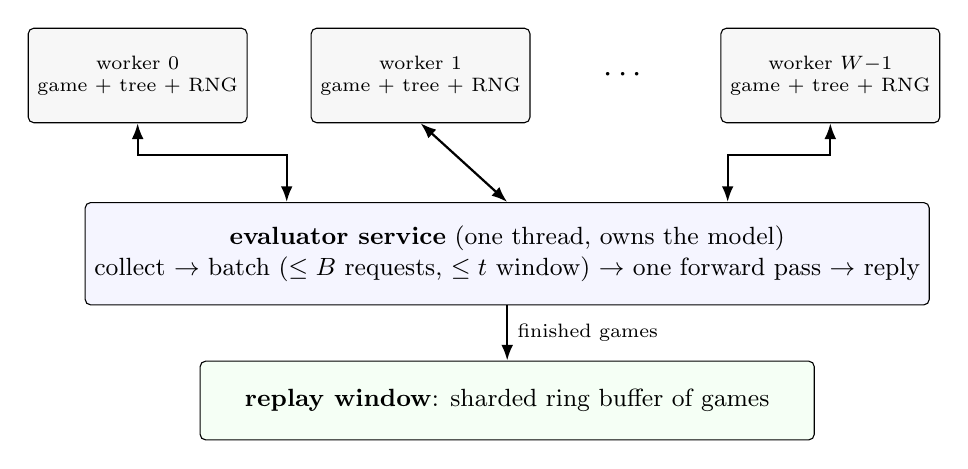
\begin{tikzpicture}[
  node distance=6mm and 8mm,
  w/.style={draw, rounded corners=2pt, align=center, font=\scriptsize,
            minimum width=26mm, minimum height=12mm, fill=black!3},
  svc/.style={draw, rounded corners=2pt, align=center, font=\small,
              minimum width=78mm, minimum height=13mm, fill=blue!4},
  buf/.style={draw, rounded corners=2pt, align=center, font=\small,
              minimum width=78mm, minimum height=10mm, fill=green!4},
  arr/.style={-{Latex[length=2mm]}, thick},
  darr/.style={{Latex[length=2mm]}-{Latex[length=2mm]}, thick},
]
\node[w] (w0) {worker 0\\game $+$ tree $+$ RNG};
\node[w, right=of w0] (w1) {worker 1\\game $+$ tree $+$ RNG};
\node[right=of w1, font=\large] (dots) {$\cdots$};
\node[w, right=of dots] (wN) {worker $W{-}1$\\game $+$ tree $+$ RNG};
\node[svc, below=10mm of w1, xshift=11mm] (svc)
  {\textbf{evaluator service} (one thread, owns the model)\\
   collect $\to$ batch ($\le B$ requests, $\le t$ window) $\to$ one forward pass $\to$ reply};
\node[buf, below=7mm of svc] (buf)
  {\textbf{replay window}: sharded ring buffer of games};
\draw[darr] (w0.south) -- ++(0,-4mm) -| ([xshift=-28mm]svc.north);
\draw[darr] (w1.south) -- (svc.north);
\draw[darr] (wN.south) -- ++(0,-4mm) -| ([xshift=28mm]svc.north);
\draw[arr] (svc.south) -- node[right,font=\scriptsize]{finished games} (buf.north);
\end{tikzpicture}
\caption{The actor layout. Workers never touch the model, the model never sees a
tree, and the service is the only place where threads interact.}
\label{fig:actors}
\end{figure}

\subsection{The evaluator service}
\label{sec:service}

The service is one thread that owns the model and runs a loop. In outline:

\begin{lstlisting}[style=rust,caption={The batching loop. One device call per
batch, one reply per request.},label={lst:service}]
loop {
    let first = rx.recv()?;                       // block until work exists
    let mut batch = vec![first];
    while batch.len() < MAX_BATCH {               // fill the batch
        match rx.recv_timeout(WINDOW) {           // ... within a time window
            Ok(req) => batch.push(req),
            Err(_)  => break,                     // window closed: run now
        }
    }
    let out = model.forward(&batch);              // ONE device call
    for (req, res) in batch.into_iter().zip(out) {
        let _ = req.reply.send(res);              // one reply per request
    }
}
\end{lstlisting}

Five decisions are embedded in that short loop.

\paragraph{Dynamic batching with a window.} The batch is bounded by both a count
and a time. The window exists to catch the tail of the arrival process, not to
build the batch: when many workers are blocked, the batch fills to the cap
immediately and the window contributes nothing to latency. This is the point to
get right when tuning, because the two failure modes are opposite. A window that
is too long adds latency to every request without improving the batch; a window
that is too short fails to gather the requests that are already available.

A simple model makes the trade-off visible. Suppose the service takes
$\tau(b) = \tau_0 + b\,\tau_1$ for a batch of $b$ (a fixed launch cost plus a
per-item cost), and suppose $Q$ workers are blocked waiting. If $Q \ge B$ the
batch is full, throughput is $B/\tau(B)$, and the window does not matter. If
$Q < B$ the service must decide between waiting up to $t$ to gather more requests
and running the smaller batch. Waiting is only worthwhile if the arrivals during
the wait more than compensate for the delay they add to the requests already
collected. In practice the useful rule is: \emph{size the batch cap so that a
healthy worker pool can fill it, and keep the window short}. The cap, not the
window, is the throughput knob.

\paragraph{One model, one thread.} The network lives exclusively on the service
thread. Workers send plain request structs and receive plain result structs; they
never hold a handle to a tensor, a device, or a module. This has a larger
consequence than it first appears.

In Rust terms, it means the system uses \emph{ownership} to make a class of
concurrency bugs unrepresentable, rather than \code{Arc<Mutex<Model>{}>} to manage
them at runtime. There is no reader--writer lock on the weights, so there is no
lock contention on the hottest resource; there is no question about whether
accelerator handles are \code{Send}, because none of them ever cross a thread
boundary; and replacing the model after a training phase is a single assignment
on a single thread, with no coordination protocol. The synchronization that
remains is exactly the batching that the design wants.

This is the most Rust-specific decision in the whole system, and it generalizes:
when two components must share a resource, first ask whether the resource can be
\emph{owned} by one of them and accessed by messages.

\paragraph{Replies travel inside requests.} Each request carries a one-shot
sender for its own reply. The service needs no table mapping request identifiers
to waiting parties, no correlation logic, and no cleanup for abandoned requests:
if a worker stops waiting, the send simply fails and the error is ignored. The
message is self-addressed, so the protocol cannot get out of step.

\paragraph{Bounded channels are backpressure.} The request channel is bounded. If
the device falls behind, workers block in \code{send} rather than accumulating an
unbounded queue of stale requests, and the system throttles itself to device
speed with no watchdog, no adaptive rate control, and no measurement. Note the
interaction with the batching loop: a bounded channel plus a
\code{recv\_timeout} window means the service is never starved by an idle pool
and never flooded by an eager one.

\paragraph{Errors need a policy.} If the service thread panics, every worker is
blocked in \code{recv} forever and the process hangs rather than failing. Two
cheap defences are worth building: the reply channel is dropped when the service
dies, so \code{recv} on the worker side returns an error that can be propagated;
and the run loop treats a dead service as a fatal condition with a message, not
as a retryable one.

\subsection{Training, inference, and the single-device problem}
\label{sec:phased}

One accelerator must serve two clients: the evaluator service during self-play,
and the trainer during the training phase. A system can either phase them or run
them concurrently.

\emph{Continuous} operation is what AlphaZero did, on separate hardware for
self-play and training. ELF OpenGo ran it continuously on shared hardware and
reported a large throughput advantage for the asynchronous pipeline, at the cost
of two specific complications: games whose moves were produced by different
network versions, which makes the training data heterogeneous, and batch
normalization statistics that lag behind the current weights, which they fixed by
recomputing those statistics from a sample of batches at intervals
\citep{tian2019elf,ioffe2015batchnorm}.

\emph{Phased} operation alternates: generate $N$ self-play games with the
evaluator alone; run $K$ training steps with the trainer alone; play evaluation
games; repeat. The reasoning for choosing this first is straightforward. On a
single device, concurrency is not really concurrency: two clients contend on one
queue, the driver serializes them anyway but less predictably than the scheduler
would, and the batch shapes fight each other, because training wants batches of
a thousand and inference wants batches of at most a few hundred. Phasing costs
nothing in correctness, makes every number reproducible per iteration, and keeps
the first working version debuggable, which matters more than a percentage of
throughput at the point where the system has never run.

The upgrade path stays open by construction, and this is the design argument for
phasing: once the evaluator and the trainer are separate owners of separate
resources, moving to continuous operation is a scheduling change, not a rewrite.
The decision rule to write down is: go continuous when profiling shows the phase
boundaries costing more than a fixed fraction of throughput, and pay ELF's
complications deliberately, including a minimum replay size before training
starts.

\subsection{The replay window}
\label{sec:buffer}

The buffer is the only mutable structure shared between threads, so it should be
as simple as possible, and it should be sized by an argument rather than by
intuition.

The argument is about what to store. Storing \emph{positions} means storing the
encoded planes, the target distribution, and the outcome: about a kilobyte per
sample, simple, and immediately usable. Storing \emph{games} means storing the
move list and the metadata: tens of bytes per game, because the planes are
derivable. The difference is a factor of several thousand -- two million games
occupy on the order of a hundred megabytes of move lists, against terabytes for
the equivalent positions.

Storing games is the better choice for three reasons. It fits comfortably in
memory without paging. It keeps the encoding decisions mutable: if the plane
layout changes during experimentation, every stored game remains valid, whereas
stored planes are frozen at the old layout. And it puts the encoding work where
the CPU is idle: the trainer thread is device-bound, not CPU-bound, so replaying
a game through the rules engine at sampling time is nearly free, and it is the
same discipline that applies to any data pipeline -- store the raw form, encode
at the boundary.

Concurrency for the buffer follows the sharding principle already established.
Appends arrive from many workers and sampling happens on one thread. A single
mutex, or a lock-free structure, is over-engineering: a sharded ring buffer with
one mutex per shard keeps lock hold times at the level of a few instructions,
the sampler round-robins the shards, and the worst case is a slightly uneven
distribution of games rather than a correctness problem. Contention here is
measured in microseconds per game, not per sample.

Persistence should be per iteration rather than per sample: appending each
finished game to a journal file bounds a crash to the current phase, at one write
per game. A system that trains for days and loses the run to a power failure will
be rebuilt with a journal after the first incident, which is one incident later
than necessary.

\subsection{Sizing, and the one number to watch}
\label{sec:sizing}

Worker count follows from cores, not from a formula. Reserve one core for the
service thread, which is mostly idle waiting on the device but must never be
scheduled late, because a late service thread stalls every worker; reserve one
for the trainer and the operating system; give the rest to workers. On an
18-core machine that is 14 workers, and it is a starting value.

The tuning signal is a single number: \emph{evaluator queue depth}, the number of
requests waiting when the service starts a batch.

\begin{itemize}
  \item Queue consistently starving (batch sizes far below the cap): add workers,
        or lower the batch cap so that the batches that do exist complete sooner.
  \item Queue consistently flooded (the bounded channel is full and workers are
        blocking in \code{send}): the device is saturated, and extra workers only
        add latency. Remove workers, or reduce simulations per move.
\end{itemize}

This is the entire control loop, and it is deliberately a measurement rather than
a model. A worked estimate of the target throughput is useful for planning and
should be labelled as derived rather than measured. With the network of
Table~\ref{tab:scaling} at roughly $1.7$ gigarithmetic operations per evaluation,
a conservative assumption of five effective tera-operations per second gives
about $2900$ evaluations per second. At $400$ simulations per move that is about
seven moves per second across all workers, so a 50-move game completes in about
seven seconds and the system produces a few hundred games per hour. A
25{,}000-game iteration then takes on the order of two days. The precise numbers
depend on the device, and the useful conclusion is the order of magnitude: plan
for days to a first non-embarrassing agent and weeks to a strong one, and
distrust any plan more precise than that before the first measurement exists.

\subsection{Determinism}
\label{sec:determinism}

Self-play is stochastic in four places: the noise vector at the root, the
temperature sampling, the symmetry transform applied to training positions, and
the mini-batch sampling. Each should be driven by a generator that is owned by
exactly one worker, seeded from a run-level seed plus the worker index, so that
the $\text{worker} \times \text{game}$ stream can be reproduced exactly.

What can be promised depends on the backend. On a CPU backend, arithmetic is
deterministic and a fixed seed reproduces a run bit for bit. On an accelerator
backend, kernel selection and autotuning can make even the same operation produce
slightly different rounding between processes, so the promise is best-effort and
must be stated as such. This matters for one practical reason: reproducing a
strange game is by far the fastest route to diagnosing a search defect, and
reproducibility has to be designed in before it is needed. Recording the seed,
the mode, and the backend in the run journal costs nothing and converts an
unreproducible anomaly into an investigation.

\section{Training, and where the framework belongs}
\label{sec:training}

\subsection{The framework boundary}
\label{sec:framework-boundary}

The single most useful structural decision in a Rust implementation is where the
deep-learning framework is allowed to appear. Here it appears in exactly one
place: the crate that owns the network. The rules engine has no dependency on it,
the search has no dependency on it, and the parallelism layer has no dependency
on it. Data crosses the boundary as plain arrays and scalars.

The concrete flow is worth writing out, because three design decisions arrive at
the same diagram:

\begin{lstlisting}[style=plaintext,caption={The only framework-aware seam in the
system. Everything above the dotted line compiles and runs with no accelerator
present.},label={lst:seam}]
board  (rules engine: bitboards, absolute colours)
  |  encode()                          -- no framework types
  v
planes [C, 17, 17] u8   (player-relative view, border ring set)
  |  convert                           -- THE ONLY framework-aware step
  v
Tensor<B, 4> [batch, C, 17, 17]
  |  forward
  v
policy logits [batch, 225] , value [batch, 1]
\end{lstlisting}

Three properties follow, and each is a practical benefit rather than an aesthetic
one.

\emph{The search is testable without a device.} Because the evaluator trait
carries plain data (Section~\ref{sec:evaluator}), the entire search can be built
and verified against a deterministic mock evaluator, on a machine with no
accelerator, before any network code exists. This is the difference between
debugging a search and debugging a search and a network simultaneously.

\emph{Compile times stay usable.} A framework and its backend machinery are heavy
dependencies. Confining them to one crate keeps incremental builds of the
frequently edited crates fast, which matters over a project measured in months.

\emph{The relative view is derived, never stored.} The engine stores absolute
colours, because the Swap2 opening does not alternate players
(Section~\ref{sec:solved}); the encoder produces the player-relative planes,
which halves the state space the network must learn. Mixing the two is a
well-known source of subtle bugs, and separating them physically -- different
crate, different types -- makes mixing them a compile error rather than a
misread.

\paragraph{Planes and the border ring.} A detail of the encoding carries more
learning consequence than its size suggests. The board is $15\times15$, but the
encoded planes are $17\times17$, with an extra ring of cells whose contents are
set to the \emph{opponent} for every position. The reason is convolutional
symmetry: with a border, a same-padding convolution at an edge cell sees a wall
of opponent stones, which is how a wall really constrains a line, instead of
seeing zeros and having to learn what an edge means. The border is a property of
the encoding layer and not of the engine's storage, so the engine keeps
$15\times15$ semantics throughout. The policy head still emits 225 logits, one
per real cell, so border cells can never become move targets.

One invariant makes this safe, and it is testable: the border ring is invariant
under the board's dihedral group, and the symmetry transforms are defined on the
$15\times15$ board, so encoding commutes with every transform. Applying a
transform and then encoding must equal encoding and then applying the transformed
transform. That property test catches an entire class of augmentation bugs,
including the ones that only affect one of the eight transforms.

\subsection{Backend genericity, and why it is not ceremony}
\label{sec:backends}

Training code should be generic over an autodiff backend; inference code should
be generic over a plain backend. In Burn's type system that means a model written
as \code{Module<B: Backend>}, instantiated during training with
\code{Autodiff<B>} to obtain gradients and during inference with \code{B} alone.
The binary fixes the concrete choice -- on a CPU-only path, the pure-Rust
\code{Flex} backend; with an accelerator feature enabled, the GPU backend.

Generic backends are usually presented as portability. The real benefit here is
\emph{testing}. Two gates depend on it directly.

The \emph{overfit test} is cheap on a CPU backend and proves the loss, the
encoding, and the training loop are wired together correctly: take a handful of
positions, train on them alone, and require the policy accuracy to approach
certainty. A loop that cannot overfit a few dozen samples has a defect that no
amount of training data will fix.

The \emph{backend parity test} is the executable form of a genuine risk. The same
weights and the same batch, evaluated on the CPU backend and on the accelerator
backend, must agree to within a small tolerance on the forward pass -- and, more
importantly, one full training step must produce parameter deltas within a
relative tolerance. Forward agreement alone does not establish that gradients or
optimizer updates are correct on the accelerator. Until the parity test passes,
training belongs on the CPU backend; once it passes, accelerator training is a
measured claim rather than an assumption. Deterministic-operation concerns on
accelerators, including non-deterministic autotuning, are the reason the
tolerance is a tolerance and not an equality.

\subsection{The training loop}
\label{sec:loop}

The AlphaZero training step needs a manual loop rather than a supervised-training
helper, for two reasons that are properties of the data and not of the
framework. Samples do not exist until they are generated: a mini-batch is
assembled by drawing games from the replay window, replaying each to a random
ply, encoding, and applying augmentation, all during training. And the policy
target is a full distribution over a masked action set, not a class index. Both
are ordinary in AlphaZero and both are outside the shape a supervised trainer
expects.

The loop is therefore: draw a game, replay it to a ply, encode, augment, and
repeat until the batch is full; forward; compute the loss; backward; step. The
only subtlety worth naming is that the augmentation transform must be applied to
the input planes \emph{and} to the policy target consistently, and that a move
index must be remapped through the same transform. Applying the transform to the
board but not to the target distribution is a silent corruption: the loss still
decreases, and the network learns a consistently permuted policy.

\subsection{The loss in practice}
\label{sec:loss-practice}

Equation \eqref{eq:alphazero-loss} becomes three pieces of ordinary code.

The value term is a mean squared error between the value head's output and the
scalar $z$, which takes values in $\{-1,0,+1\}$.

The policy term is a cross-entropy against a \emph{soft} target, which is the one
place a standard loss function cannot be used directly, because most
cross-entropy implementations take a class index. The expression is

\begin{equation}
\mathcal{L}_{\text{pol}}(\pi, p) \;=\; - \sum_{a \in \mathcal{A}_{\text{legal}}}
\pi_a \log p_a ,
\end{equation}

where $p$ is the softmax of the network's logits over the legal actions. Compute
it as \code{-(pi * log\_softmax(logits)).sum()} for numerical stability, and
restrict the sum to legal actions, which is the same masking discipline as
Section~\ref{sec:expand}: the target $\pi$ is already zero on illegal cells, but
an explicit mask keeps a bug in the target construction from silently leaking
mass.

The regularization term is normally not written in the loss at all but expressed
through the optimizer, which brings the next decision.

\subsection{Optimizer and schedule}
\label{sec:optimizer}

The primary sources train with stochastic gradient descent and momentum $0.9$,
with an $L_2$ penalty of $10^{-4}$ inside the loss and a step-decay learning-rate
schedule \citep{silver2017alphagozero,silver2018alphazero}.
Neither paper explains the choice, which is itself informative: in 2017 the
recipe for a deep residual network was SGD with momentum and step decay, and the
architecture was chosen to match the state of the art in image recognition
\citep{he2016resnet}. The optimizer came with the architecture, and every major
replication kept it \citep{tian2019elf,wu2019katago}.

For a single-device run at a much smaller batch size, AdamW
\citep{kingma2014adam,loshchilov2017adamw} is a defensible substitute, and the
reason is worth stating precisely so that the substitution is not mistaken for a
free improvement. With SGD, an $L_2$ penalty in the loss and decoupled weight
decay are nearly the same mechanism, differing by a learning-rate factor. With
Adam they are not the same at all, because the penalty's gradient passes through
the adaptive preconditioner; that difference is the AdamW result. So the
mechanism the papers rely on -- a weight-decay rate of $10^{-4}$ acting as a
smoothness control on a search-critical function
(Section~\ref{sec:loss}) -- can be preserved under AdamW by using decoupled
decay. The reasons to prefer adaptive methods at small scale are the standard
ones: faster early convergence and far less sensitivity to the learning rate.
The reason the papers did not need them is the standard counter-argument:
adaptive methods have been reported to generalize worse on image-classification-
style tasks, and training on a distribution that never stops moving is a
generalization problem throughout the run \citep{wilson2017adaptive}.

Both choices should be configuration, not a rewrite, so that a fidelity
experiment is a one-line change.

The learning-rate schedule needs the same treatment. AlphaGo Zero stepped
$10^{-2} \to 10^{-3} \to 10^{-4}$; AlphaZero started at $0.2$ and dropped three
times, in step with a doubled batch size. Those schedules are tuned for SGD at
batches of two to four thousand and do not transfer to a batch of a thousand with
an adaptive optimizer. A linear warmup followed by cosine decay is the more
useful starting point, and the specific numbers are an experiment, not a
citation.

\subsection{Records, checkpoints, and one trap}
\label{sec:records}

Checkpointing a model in a reduced-precision format is a standard space
optimization and a bad idea in this system. If candidate and baseline are
compared by playing games against each other, and the candidate's weights have
been rounded to half precision while the baseline's have not, the comparison
measures quantization noise as well as training. Precision loss of that kind is
exactly the size of the differences the arena is trying to resolve. The rule is
therefore: store models at full precision.

Checkpoint often, and keep the checkpoints. A run measured in days should never
lose more than one iteration to a fault, and disk is cheaper than a week of
compute.

\subsection{Verification gates}
\label{sec:gates}

The order of the following gates matters, because each one makes the next one
meaningful.

\begin{enumerate}
  \item \textbf{Rules engine, differentially.} A fast bitboard implementation
        against a naive array implementation, on ten thousand random games,
        compared ply by ply. Any disagreement is a defect in one of them.
  \item \textbf{Search, against known facts.} Tactical puzzles with verifiable
        solutions, driven by the deterministic mock evaluator: a win in one must
        be found at a small simulation budget, forced blocks must be played,
        short forced sequences must be found. This is the test that catches the
        sign convention of Section~\ref{sec:backup}.
  \item \textbf{Prover soundness.} Every emitted line is re-verified by replaying
        it while enumerating all defender alternatives. On shallow positions,
        brute-force adjudication must agree with every proof claim. The prover
        may miss wins; it must never certify one that is not there.
  \item \textbf{Network shapes and overfitting.} Forward shapes on both backends,
        and the overfit test of Section~\ref{sec:backends}.
  \item \textbf{Backend parity.} One full training step, both backends,
        parameter deltas within tolerance.
\end{enumerate}

Nothing trains at length until gate 5 passes. The reason is that the failure it
detects -- a correct-looking forward pass with wrong gradients -- produces a run
that looks normal, costs days, and produces a weak agent. That failure is
indistinguishable from a bad hyperparameter at the point where it is observed,
which is why it must be excluded early and mechanically.

\section{Closing}
\label{sec:closing}

\subsection{The chain, in one page}

The mathematics begins with an expectation over trajectories
\eqref{eq:objective} and makes its gradient estimable without a model of the
environment \eqref{eq:reinforce}. The policy gradient theorem then replaces the
trajectory return with a state--action value, at the price of weighting by the
policy's own state distribution \eqref{eq:pgt}. Substituting a learned value
gives the actor--critic family, and the choice of how to train that value decides
the stability of everything above it: bootstrapping buys sample efficiency and
risks divergence.

In the deterministic branch, the same identity survives without the action
integral \eqref{eq:dpg}, which makes continuous control tractable; that branch is
where the deep deterministic policy gradient lives, and it is not the branch that
produced AlphaGo.

The AlphaGo branch replaces the gradient estimator entirely. Policy improvement
becomes tree search; policy evaluation becomes regression on the outcome of games
played by the improved policy; the network is refitted to both. The result is an
approximate policy iteration whose two operators are a learned function and a
search built on top of it, and its theoretical frame is Expert Iteration. The
bandit results supply the selection rule and the only real guarantees in the
system, and the guarantees stop where the learned prior begins.

The engineering has two hard problems, and they are the same problem seen twice:
a tree that owns its children in a language where recursive ownership is
expensive to express, and a single accelerator that must serve many cheap,
irregular searches. The answers are a flat arena with integer indices, and many
independent trees feeding one batching service. Both answers trade a
compile-time guarantee for a stated invariant, and both are worth the trade
precisely because the invariants are small enough to write down
(Section~\ref{sec:invariants}).

\subsection{What is guaranteed, and what is measured}

The system that this monograph describes is an empirically justified system. It
contains, at its centre, three components with no convergence proof: PUCT with
learned priors, approximate policy iteration with deep function approximation,
and the self-play loop itself (Table~\ref{tab:proven}). Every one of them worked,
in the primary sources and in several independent replications, and none of them
comes with a theorem.

That is not a defect to be fixed; it is the normal state of deep reinforcement
learning, and it has one practical consequence that shapes the engineering more
than any theoretical consideration: correctness must be established against
known facts rather than by appeal to theory. Gomoku is unusually generous in this
respect. Positions with exact values and forced-win sequences with mechanical
verification are available without any learning, and they can be used to test
the search, the prover's soundness, and the sign conventions before a single
gradient is computed. A system that passes those tests is still not proven
correct, but it is anchored to ground truth at the points where defects are most
likely and most expensive.

\subsection{The decisions that are expensive to reverse}

Three choices in this monograph are worth more thought than the rest, because
they are the ones that are painful to change later.

\emph{The tree representation.} A flat arena with integer indices is not
elegant, and it gives up a compile-time guarantee. It is chosen because the
alternative representations either do not compile or pay runtime costs in the
hottest loop in the system. Everything that touches the tree -- traversal,
backup, reuse across moves, serialization for debugging -- is written against
this representation, so changing it later is a rewrite of the search crate.

\emph{Ownership of the model.} Making the network a single owner on a single
thread, with plain messages as the interface, removes an entire class of
concurrency problems from the design rather than managing them. The alternative
-- shared weights behind a lock -- looks simpler in the first ten lines of code
and is worse in every line after that.

\emph{What the replay window stores.} Storing games rather than encoded positions
keeps the encoding decisions mutable and reduces memory by orders of magnitude.
It also means the corpus remains valid while the plane layout is still being
experimented with, which is exactly the period during which the corpus is
growing.

\subsection{The order of the upgrades}

Section~\ref{sec:proven} argues that the guarantees live in the skeleton, and
Section~\ref{sec:scaling} transfers the published constants to a smaller problem.
The natural next step is to change things, and the order matters, for one
structural reason: some upgrades change the distribution of the training data and
others do not. A change of the data distribution cannot be evaluated against a
baseline whose data came from a different distribution, so such changes must come
after a clean, working baseline exists, and must be made one at a time.

The upgrades that leave the data distribution alone can be made early: growing
the network, adding pooling to the heads, moving from phased to continuous
execution, and improving the evaluation setups. The upgrades that change the data
distribution -- sampling some moves with a smaller search budget, adding
auxiliary prediction targets, changing the temperature schedule, changing the
simulation count -- must wait, and must be measured against a frozen baseline by
playing games rather than by watching the loss.

The general rule is the one every part of this monograph has followed: decide
what can be decided by argument, measure what cannot, and keep the set of things
being changed at once to one.

\subsection{Reading the primary sources}

The three papers reward being read in sequence rather than separately, because
the deletions of Table~\ref{tab:removals} are the argument. For the
mathematics, the policy gradient theorem and the deterministic policy gradient
papers are short and worth their length; Expert Iteration names the two moving
parts of the loop; and the UCT and PUCT papers are the two ends of the search
argument, including the place where its guarantee stops.


\appendix
\section{Notation}
\label{app:notation}

\begin{table}[h]
\centering
\small
\begin{tabularx}{\textwidth}{@{}l X@{}}
\toprule
Symbol & Meaning \\
\midrule
$\mathcal{S}, \mathcal{A}$ & sets of states and actions (positions and moves) \\
$P(s' \mid s, a)$ & transition kernel; deterministic for a board game \\
$\gamma$ & discount factor; $\gamma = 1$ for a game with terminal outcome \\
$r, z$ & per-step reward, and the final outcome $z \in \{-1,0,+1\}$ \\
$\rho(s_0)$, $d^\pi(s)$ & start-state distribution, and the discounted
state-visitation distribution under $\pi$ \\
$\pi_\theta(a \mid s)$ & stochastic policy with parameters $\theta$ \\
$\mu_\theta(s)$ & deterministic policy \\
$v^\pi(s)$, $Q^\pi(s,a)$ & state value and state--action value under $\pi$ \\
$G_t$ & return-to-go from step $t$ \\
$J(\theta)$ & the objective; expected outcome of the initial states \\
$b(s)$ & baseline in the REINFORCE estimator \\
$f_\theta(s) = (p, v)$ & the network: raw policy $p$, value $v = \E[z \mid s]$ \\
$P(s,a)$, $N(s,a)$, $W(s,a)$, $Q(s,a)$ & prior, visit count, value sum, and mean
value of an edge in the search tree \\
$U(s,a)$ & the PUCT exploration bonus \\
$c_{\mathrm{puct}}$ & PUCT exploration constant \\
$\eta \sim \mathrm{Dir}(\alpha)$ & Dirichlet noise vector at the root \\
$\varepsilon$ & noise mixture weight \\
$\tau$ & sampling temperature \\
$\pi_a$ & the improved policy: normalized root visit counts; the policy training
target \\
$\mathrm{NodeId}, \mathrm{EdgeId}$ & integer indices into the search arena \\
$w$ & one arena node's value sum, accumulated from the chooser's perspective \\
$\tau_0, \tau_1$ & fixed and per-item cost of one batched evaluation \\
$B$, $t$ & batch cap and collection window of the evaluator service \\
\bottomrule
\end{tabularx}
\caption{Symbols used throughout. Each is redefined at first use in the body.}
\label{tab:notation}
\end{table}

\paragraph{Key numbered relations.}

\begin{itemize}
  \item \eqref{eq:objective}: the objective.
  \item \eqref{eq:reinforce}: the REINFORCE gradient estimator.
  \item \eqref{eq:pgt}: the policy gradient theorem.
  \item \eqref{eq:td}: the temporal-difference error.
  \item \eqref{eq:dpg}: the deterministic policy gradient.
  \item \eqref{eq:ucb1}: the UCB1 selection rule.
  \item \eqref{eq:puct}: the PUCT selection rule.
  \item \eqref{eq:alphazero-loss}: the AlphaZero loss.
  \item \eqref{eq:throughput}: self-play throughput.
\end{itemize}


\bibliographystyle{plainnat}
\bibliography{refs}

\end{document}
